%chapter-05.tex
\chapter{Evaluation} 

In this chapter, we will evaluate the performance and effectiveness of our Rapid Recovery Desktop system. In terms of performance, we breakdown the overhead of the entire system and quantify the impact of virtualization and enforcement elements (FS-VM and NET-VM). In terms of effectiveness, we do an analytic evaluation of protection against various types of malware. Finally, to further evaluate effectiveness, we include an evaluation of the recovery properties of the system.

\section{Performance}

The performance of the system can be broken down into two main categories: (1) the overhead of virtualization and (2) the overhead of enforcement. We describe these performance overheads in the next two sections (\ref{sec:virt-overhead} and \ref{sec:enforce-overhead} respectively).

\subsection{Virtualization Overhead}
\label{sec:virt-overhead}

As was already discussed in Section \ref{sec:related-history-evolution}, we expect that hardware support for virtualization will eventually reduce the overhead due to virtualization to a negligible amount. However, current commodity desktop systems still do experience a fair amount of overhead due to running in a virtualized environment. This overhead varies significantly based on the type of virtualization, the operating system, and the workload. In this section, we show some specific results that demonstrate this overhead.

We break down the virtualization overhead in terms of disk and network. We have taken a variety of measurements on virtualization systems over the years and include further details of some of those studies in Appendix A. For the purposes of evaluating our prototype system, we focus specifically on a wide range of tests using the KVM hypervisor, leaving a similar Xen hypervisor analysis as future work. We chose to focus first on KVM since we hope to make early use of the open source Spice VDI frontend that improves video and mouse performance of virtual machine. Recall that there is a version of qemu/KVM-spice which we discussed in \ref{sec:vmm-implementation}. We expect that Xen will have similar or perhaps, in some cases, better performance than KVM. Xen will also likely be able to support Spice in the future, which requires Xen QEMU support and Spice QEMU support to be properly integrated.

We ran our disk and network tests on the QEMU-KVM hypervisor version 0.12.3, which is included in Fedora 13. Our hardware provides first generation virtualization support, namely Intel VT-x and is a Dell OptiPlex 745 with a 2.4 GHz Intel Core 2 CPU 2200, 250 GB hard drives, and 4GB of RAM. We tested a variety of guest types including Ubuntu, Fedora, Windows XP, and Windows 7. In this section we provide specific analysis of the results most relevant to this dissertation. In appendix A, we discuss some of the results in more detail and describe how to obtain the raw performance results.

\subsubsection{Virtual Disk I/O Overhead}
To test disk I/O, we use IOzone version 3\_347 compiled from source on each platform respectively. For each platform we report read and write performance to an 8GB file for a range of block sizes. Figures \ref{fig:linux-read} and \ref{fig:linux-write} demonstrate that the read and write performance for Linux guests is quite good. In particular, the read performance in Figure \ref{fig:linux-read} shows that for Linux guest reads to an 8GB file have a (16\% on average) better read performance than native (Linux base), which is likely due to the write-through cache that KVM uses by default. For Linux write performance (Figure \ref{fig:linux-write}), the average degradation compared to native is 19\%. On the other hand, Windows guest read and write performance is not very good.  As shown in Figures \ref{fig:windows-read} and \ref{fig:windows-write}, the average degradation on a Windows guest compared with Windows Native is 41\% for reads and 94\% for writes. While we believe many end users will be better served by a safer system even if it is slower, this is substantial and could dissuade end users. Most desktop users have Windows installed, so they may want Windows guests rather Linux guests.

\begin{figure}[tbp]
\begin{centering}
\rotcaption{Linux guest read performance}
\label{fig:linux-read}
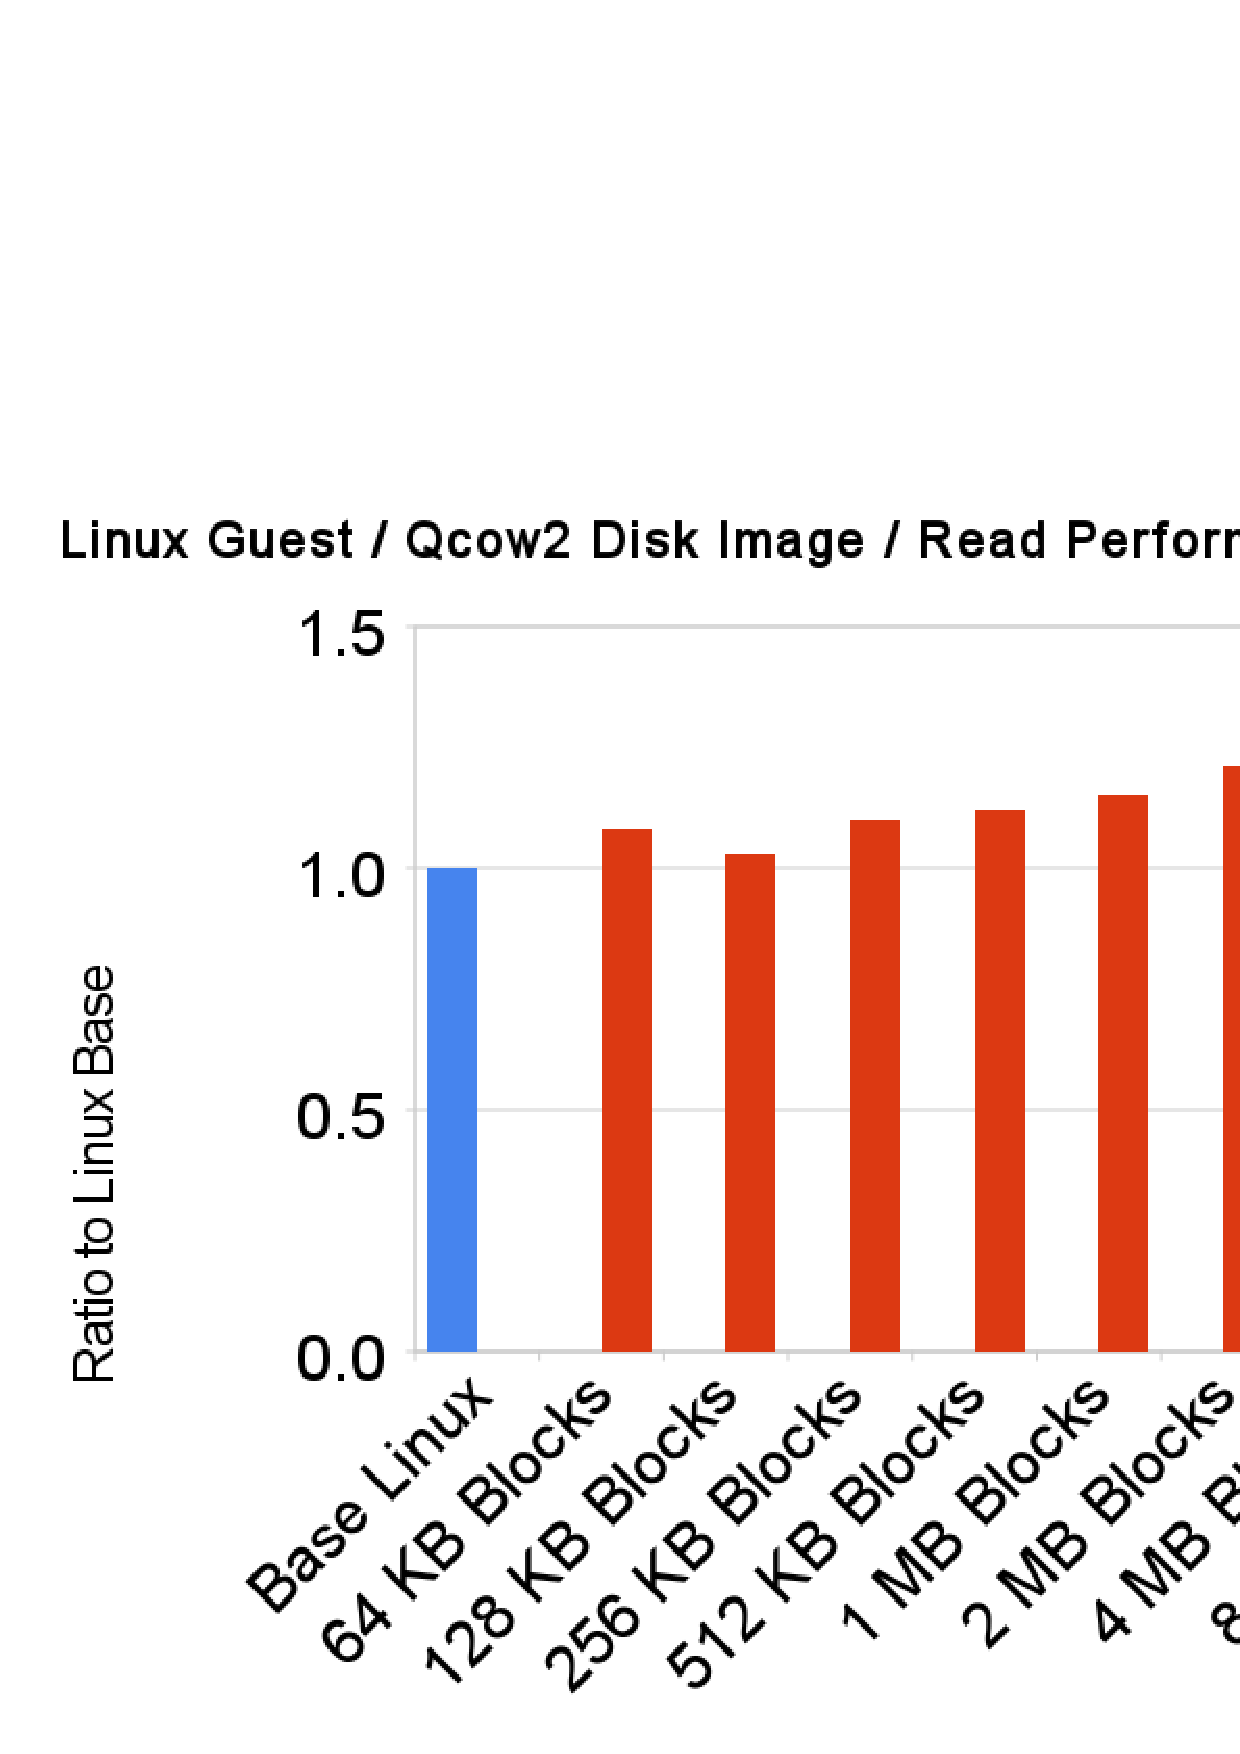
\includegraphics[scale=.7,angle=90]{figs/linux-read}
\end{centering}
\end{figure}

\begin{figure}[tbp]
\begin{centering}
\rotcaption{Linux guest write performance}
\label{fig:linux-write}
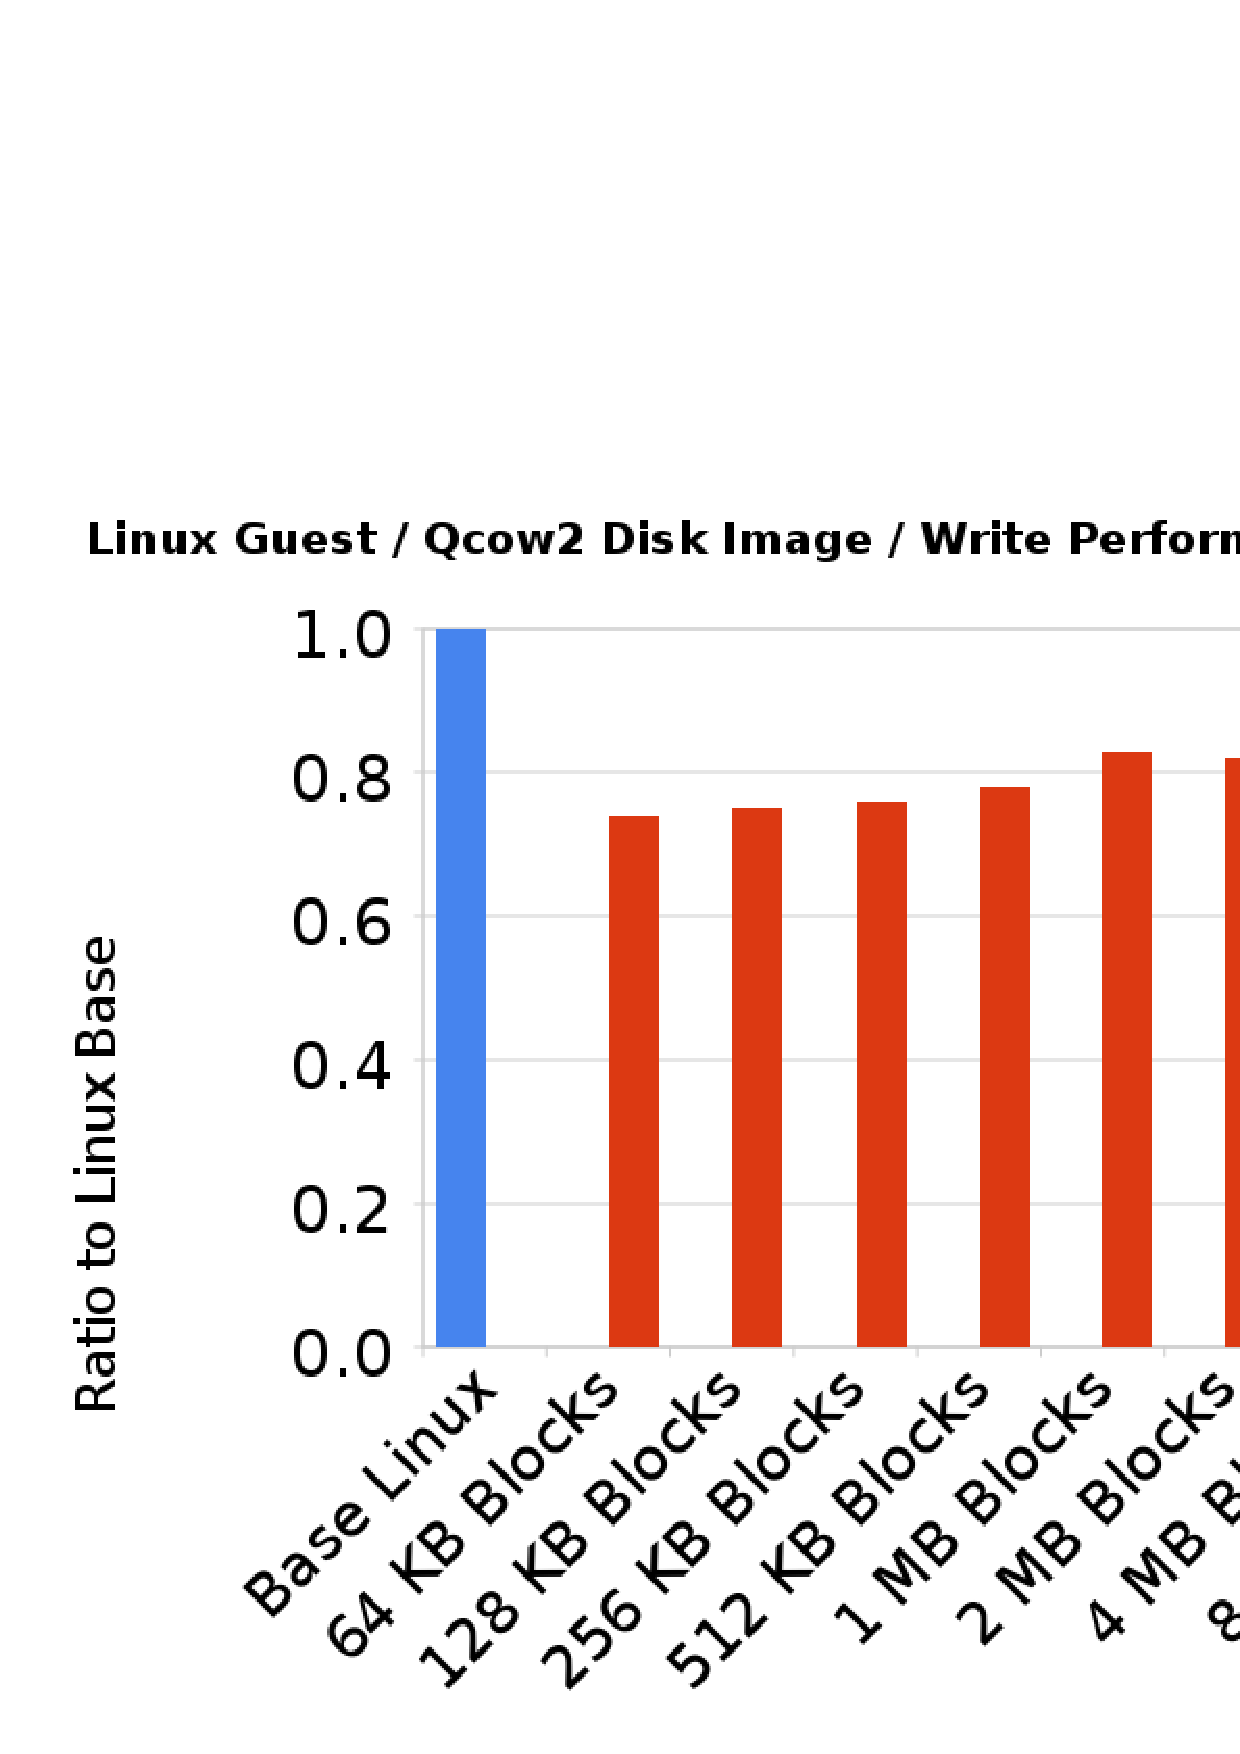
\includegraphics[scale=.7,angle=90]{figs/linux-write}
\end{centering}
\end{figure}

\begin{figure}[tbp]
\begin{centering}
\rotcaption{Windows guest read performance}
\label{fig:windows-read}
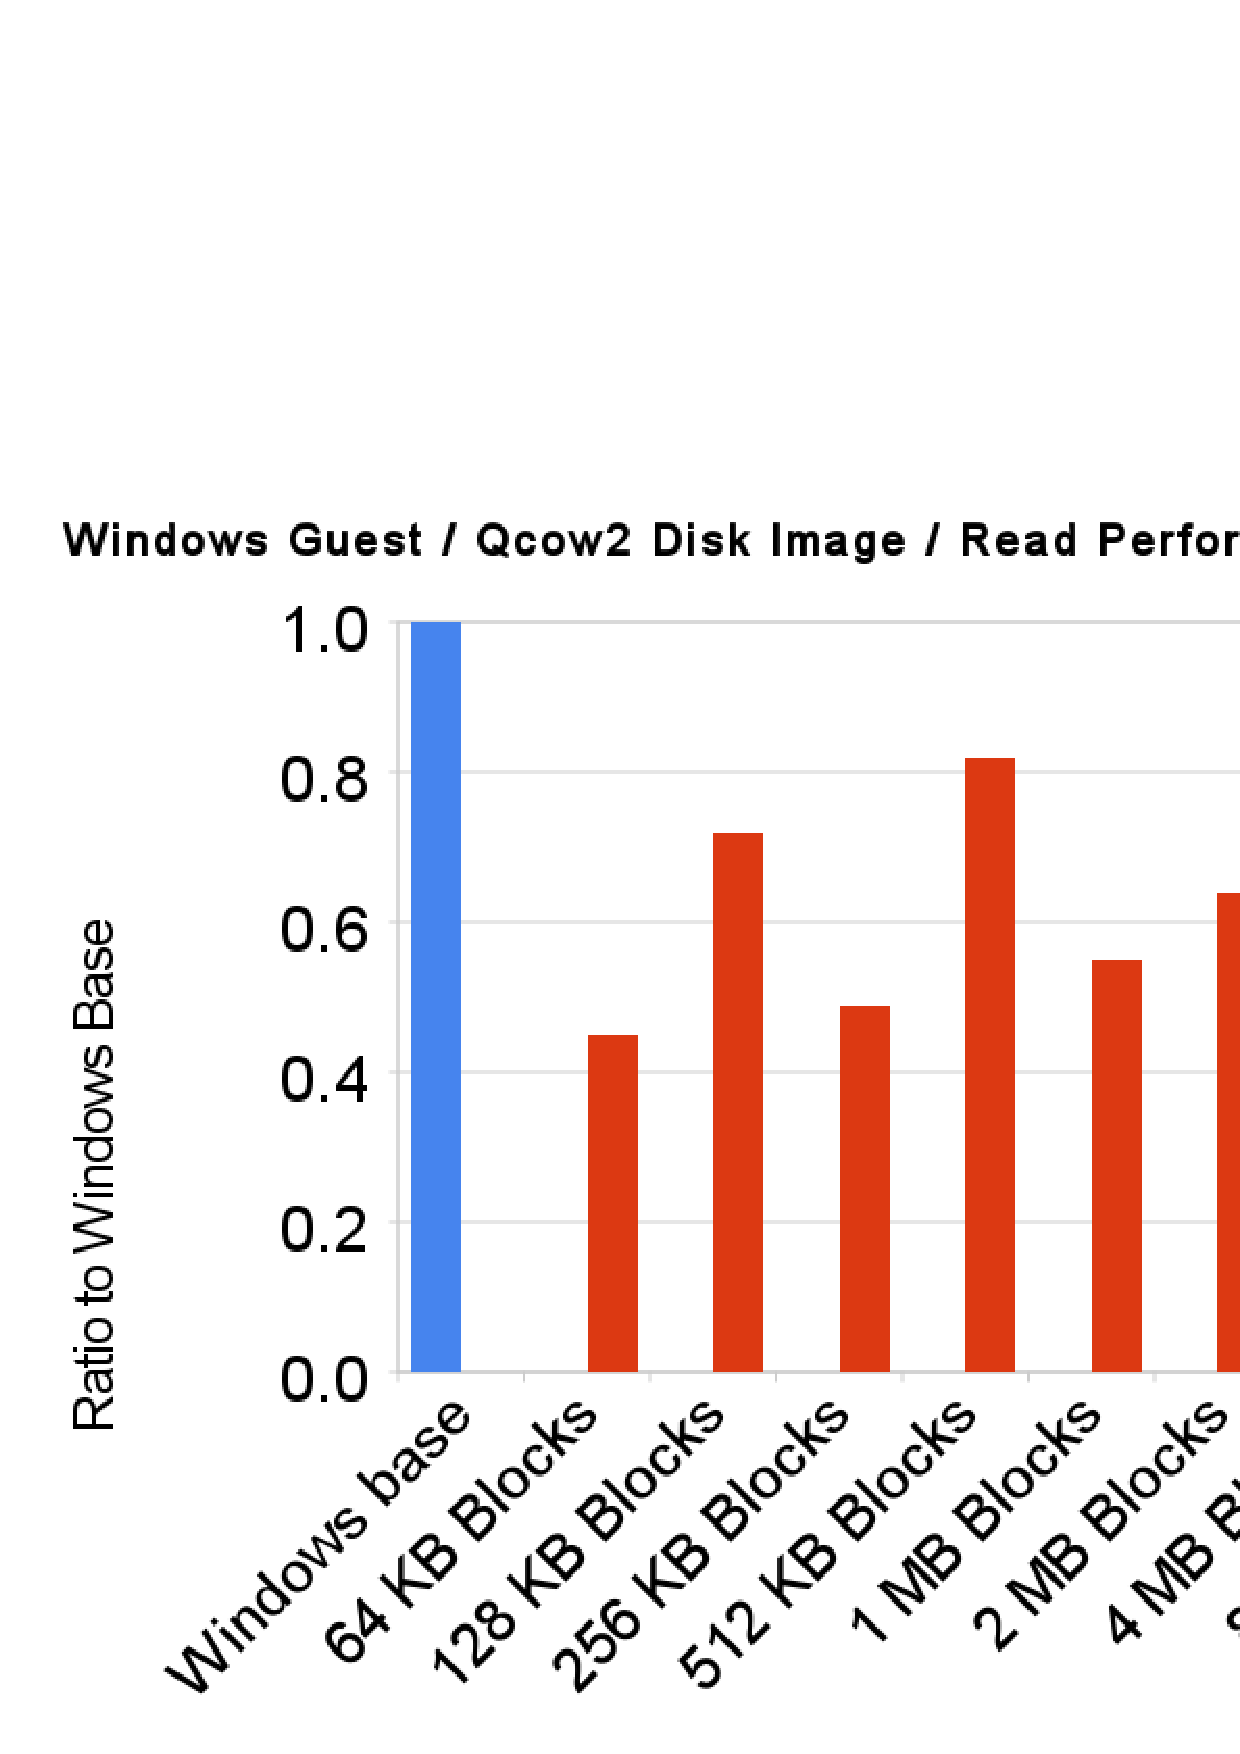
\includegraphics[scale=.7,angle=90]{figs/windows-read}
\end{centering}
\end{figure}

\begin{figure}[tbp]
\begin{centering}
\rotcaption{Windows guest write performance}
\label{fig:windows-write}
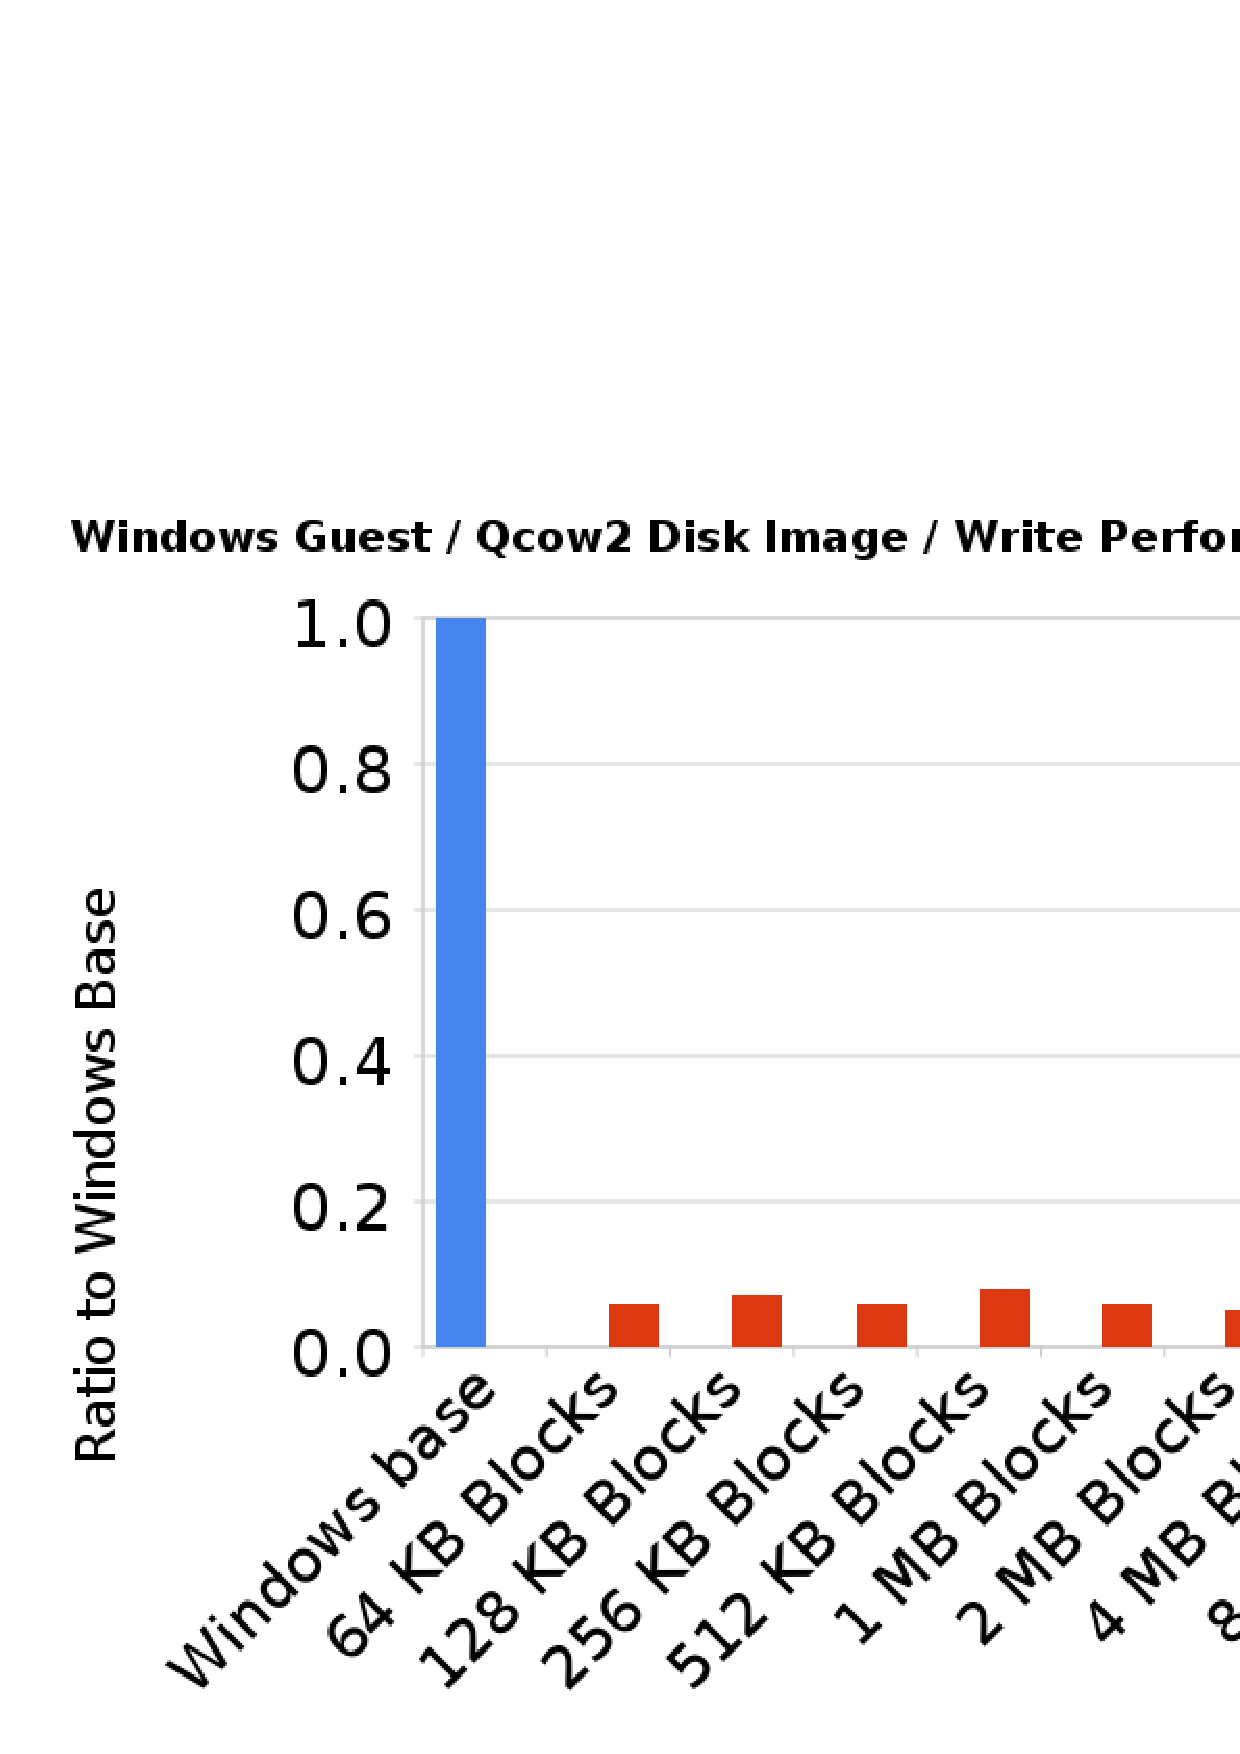
\includegraphics[scale=.7,angle=90]{figs/windows-write}
\end{centering}
\end{figure}

We looked into ways to improve the Windows guest I/O performance and found that the most common way to improve performance is to use a different virtual disk backend. It is well known that moving from a flexible disk format to something more rigid can improve performance, but is not as versatile. So, although qcow2 was our first choice, we decided to try different disk image backends. In particular, we ran the IOzone read and write tests on a raw disk image and an LVM logical volume. As is shown in Figures \ref{fig:windows-read-summary} and \ref{fig:windows-write-summary}, the average read performance improves to an average degradation of 38\% and 35\% with a raw disk image and logical volume image respectively. Similarly, write performance improves to an average degradation of 86\% and 82\% for a raw disk image and logical volume image respectively. While this is an improvement, the remaining degradation is still substantial.

\begin{figure}[tbp]
\begin{centering}
\rotcaption{Windows guest read performance using a variety of virtual disk backends}
\label{fig:windows-read-summary}
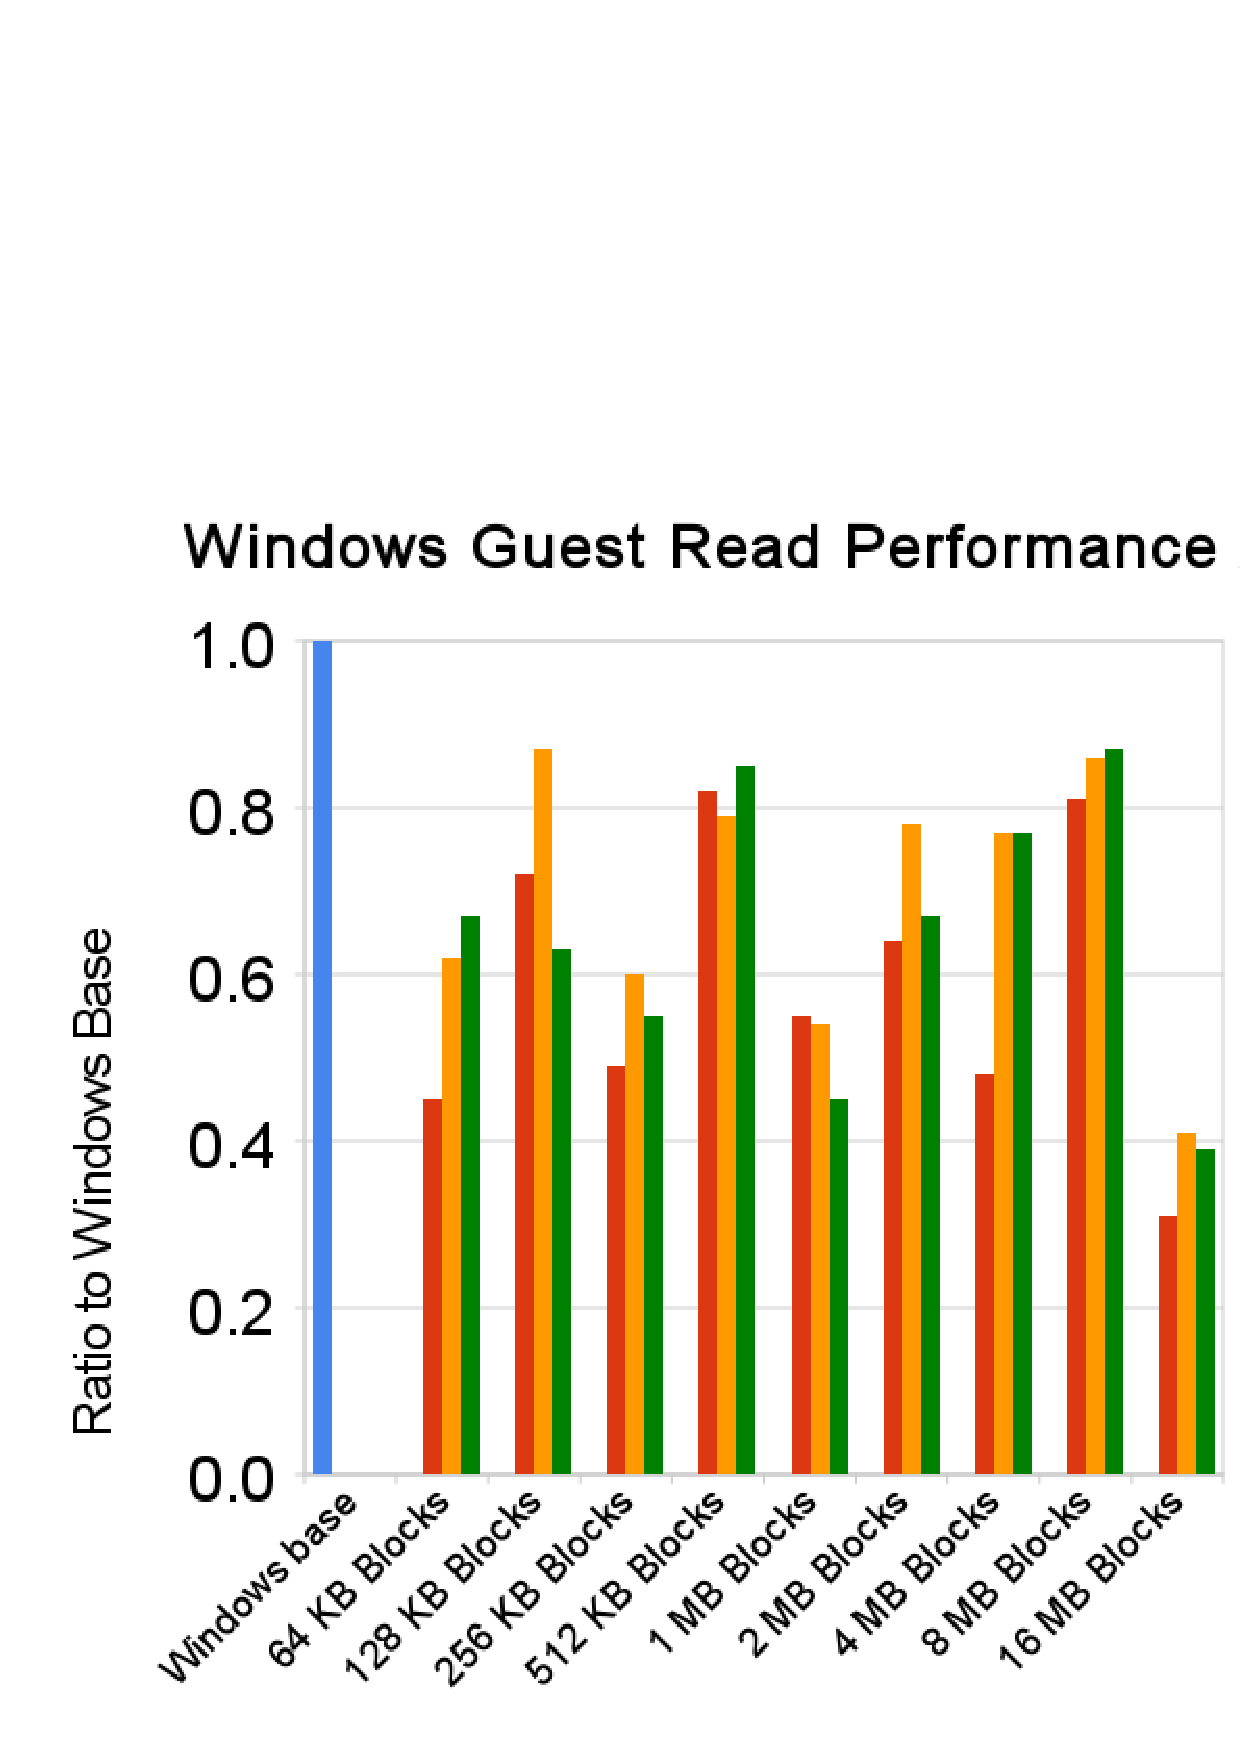
\includegraphics[scale=.7,angle=90]{figs/windows-read-summary}
\end{centering}
\end{figure}

\begin{figure}[tbp]
\begin{centering}
\rotcaption{Windows guest write performance using a variety of virtual disk backends}
\label{fig:windows-write-summary}
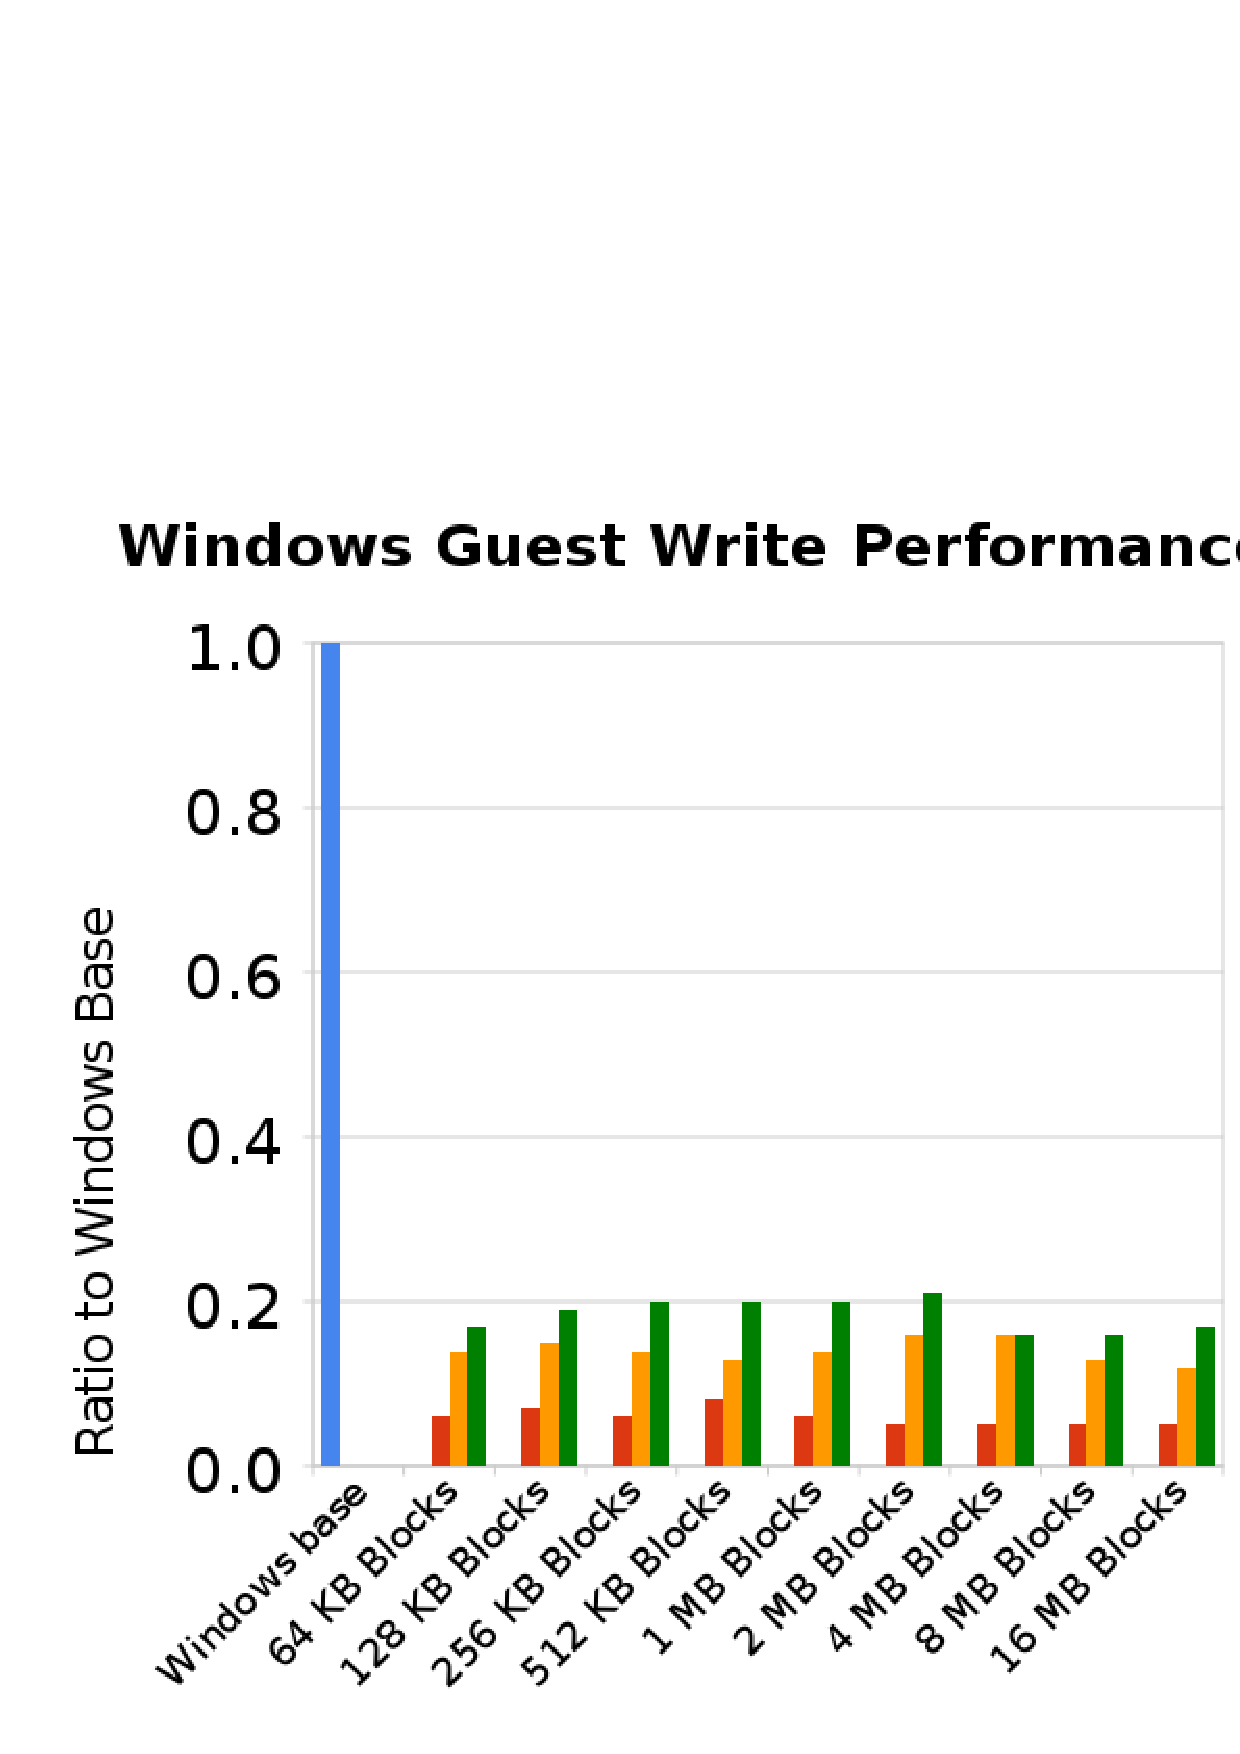
\includegraphics[scale=.7,angle=90]{figs/windows-write-summary}
\end{centering}
\end{figure}

So in summary, the disk I/O for Linux guests performs well, but future work will be needed to improve upon Windows performance. We see that the disk backend can make a modest difference. Other possible areas for improvement include I/O schedulers, Kernel Shared Memory, and using different caching strategies (for example, we could try write-back caching or no cache). The drivers for Windows guests are also likely to improve over time. So, upgrading to new drivers when they become available could help. For future work, we would also like to compare the I/O results on Xen.

\pagebreak

\subsubsection{Virtual Network Overhead}

To test the network overhead we used NetPIPE version 3.7.1 compiled on each platform respectively. All tests are taken using a cross-over cable directly connected to the physical Realtek RTL-8169 Gigabit Ethernet cards of two different physical systems. The networking used for the guest is Open vSwitch version 1.0.1. The NetPIPE bechmark tests throughput at varying packets sizes. Figure \ref{fig:linux-network} shows that the average network throughput degradation of a Linux guest compared to native (Linux base) is 30\%. Figure \ref{fig:windows-network} shows that the average network throughput degradation of Windows guest compared to native (Windows base) is 52\%.

Although there is quite a bit of network degradation, the throughput provided may still be acceptable in practice for the current desktop system use-case. The network drivers are likely to improve and optimizations for handling network are becoming available. Further investigation will be needed to determine which optimizations could fit well into our architecture. One example of improving network on the Windows platform is to increase the TCP window size\footnote{Instructions and explanation of this procedure can be found at:  http://www.linux-kvm.org/page/WindowsGuestDrivers/kvmnet/registry}.

\begin{figure}[tbp]
\begin{centering}
\rotcaption{Linux guest networking performance}
\label{fig:linux-network}
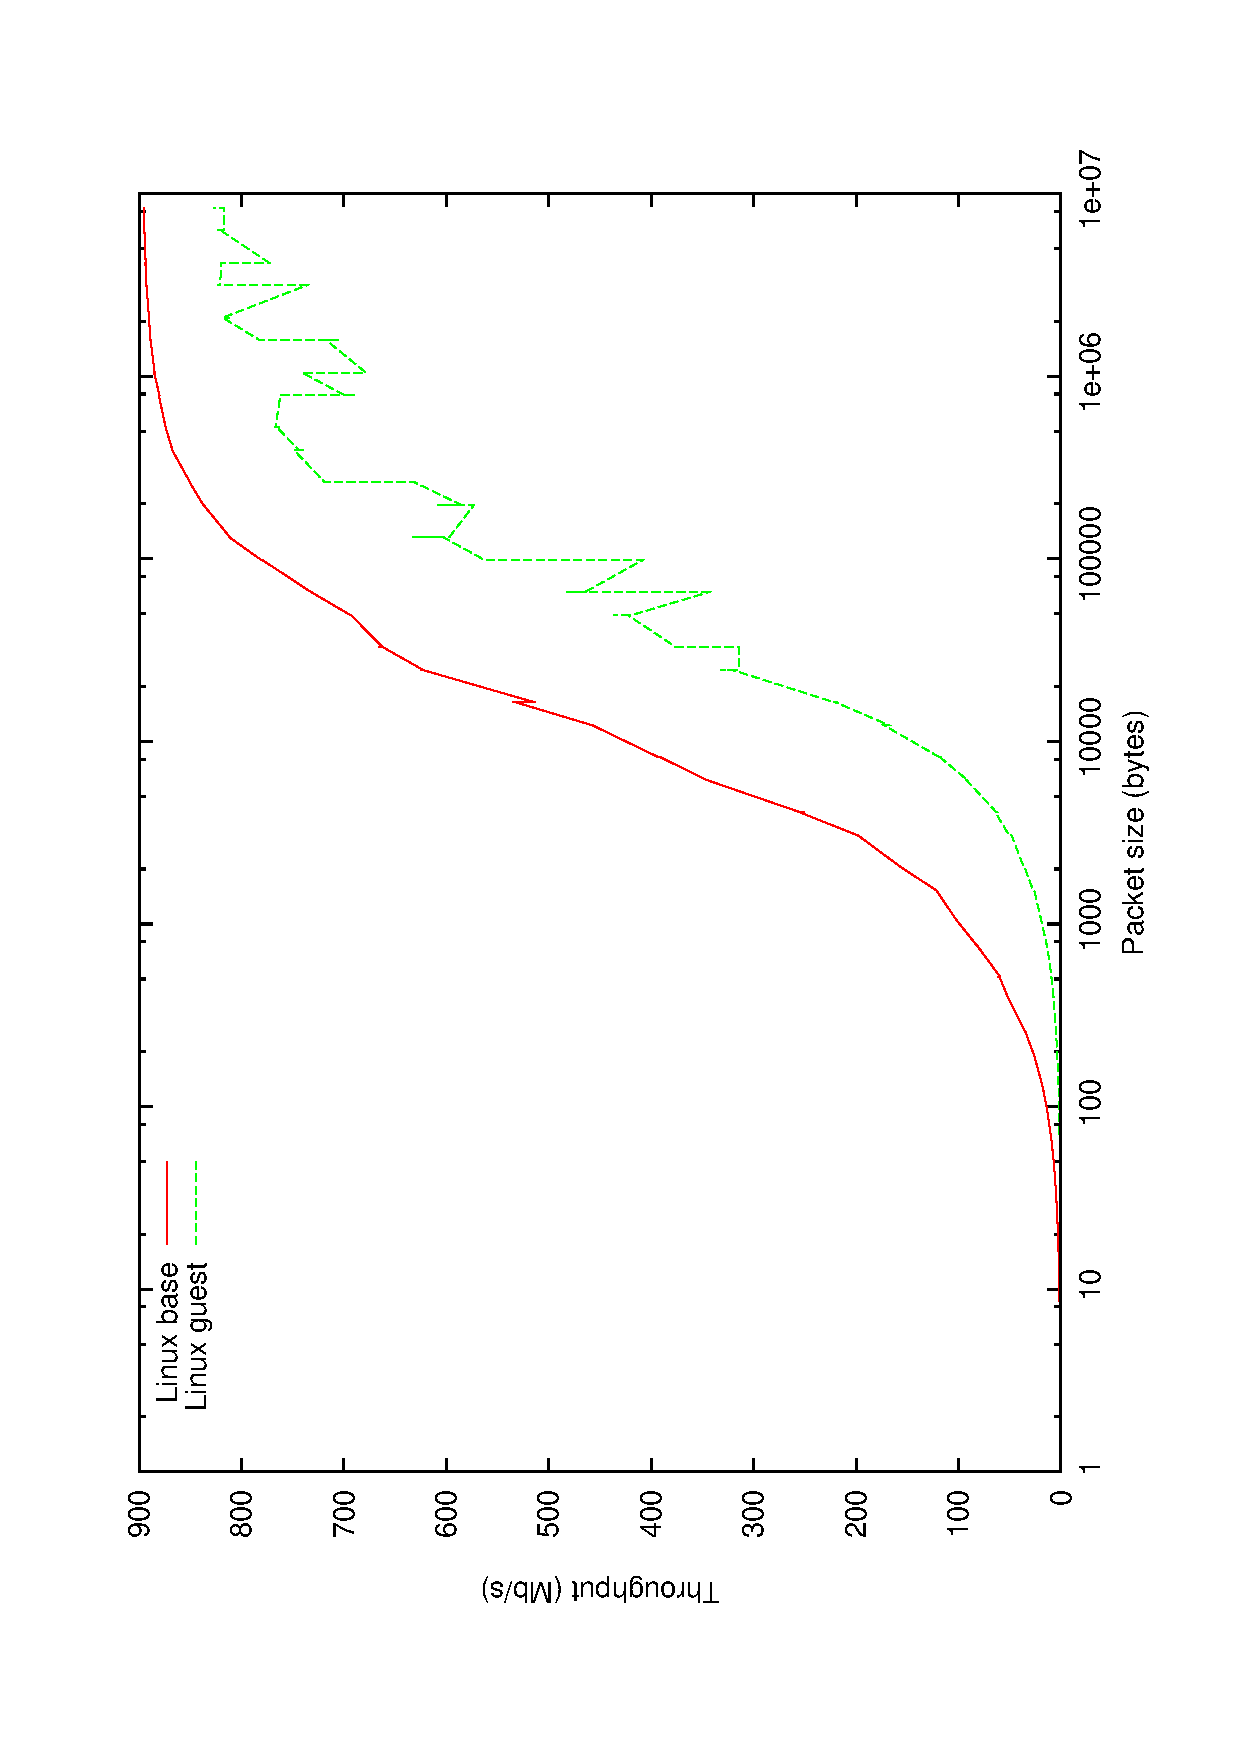
\includegraphics[scale=.7]{figs/linux-network}
\end{centering}
\end{figure}

\begin{figure}[tbp]
\begin{centering}
\rotcaption{Windows guest networking performance}
\label{fig:windows-network}
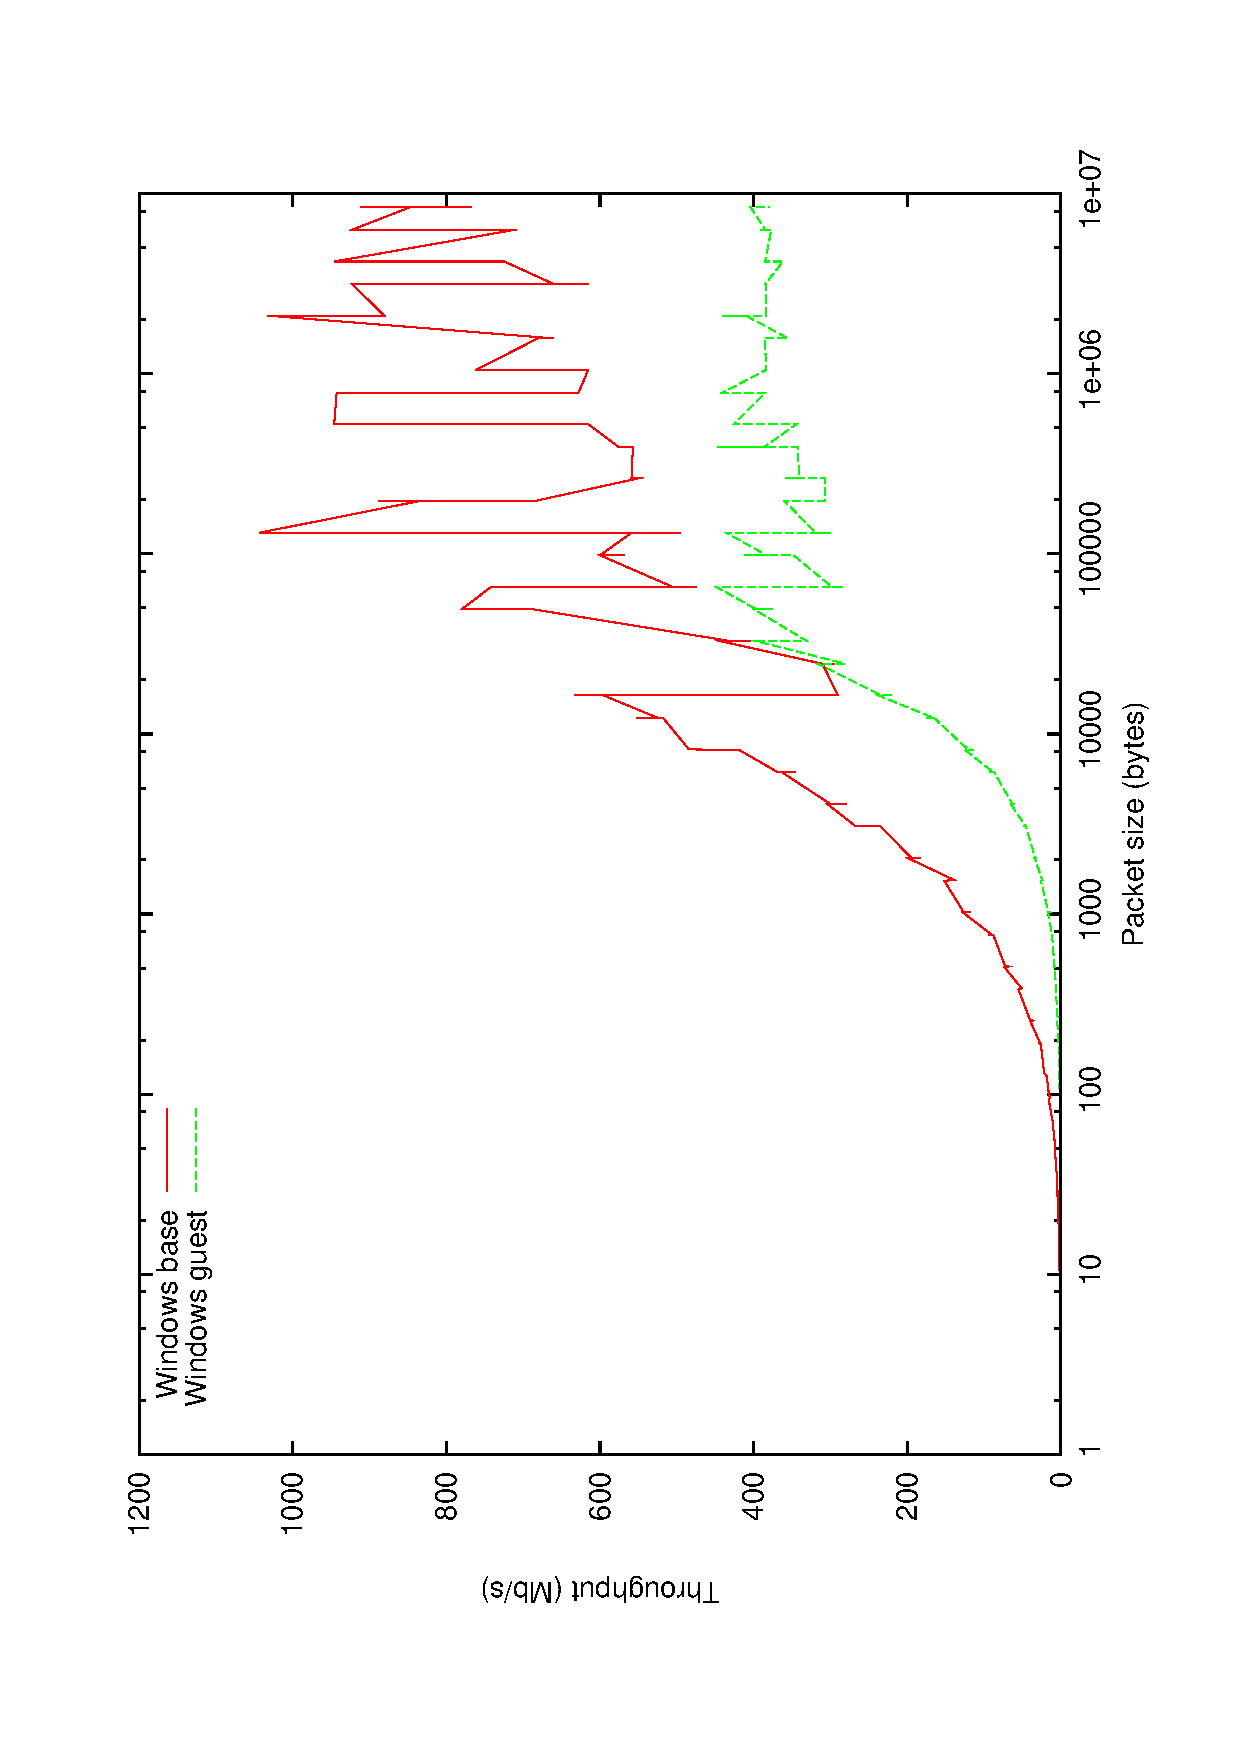
\includegraphics[scale=.7]{figs/windows-network}
\end{centering}
\end{figure}

We conclude our discussion of virtualization overhead with the fact that a typical desktop user is not likely to experience these worst case performance degradations. The majority of the target users run a simpler set of applications, for example web browsers, email clients, and word processors. These applications are not nearly as intensive as the benchmarks that are intended to push the limits and stress the system, such as IOzone and NetPIPE. In practice, we have noticed that typical web-browsing and playing a online video (such as via YouTube) is a reasonable experience. Further usability studies are a good area of future work. Also, recall that virtualization software and hardware are both improving and should eventually reach the point where virtualization overhead is negligible.

\subsection{Enforcement Overhead}
\label{sec:enforce-overhead}

The second type of overhead that we need to measure is the overhead due to adding extra enforcement to virtual appliances. The two enforcement elements that we have designed, implemented, and integrated into our system are an FS-VM and a NET-VM. To measure the performance overhead of enforcement, we put each enforcement element in place and re-ran the IOzone and NetPIPE benchmarks for the FS-VM and NET-VM respectively.

\subsubsection{FS-VM Overhead}

In our current system, the FS-VM is implemented with Samba version 3.4.7 as included in Ubuntu 10.04 Server. Figures \ref{fig:fs-vm-read} and \ref{fig:fs-vm-write} show that the average degradation added by the FS-VM is 79\% for reads and 67\% for writes. Compared to Linux base the degradation is 76\% for reads and 73\% for writes. This is significant degradation and tuning will be necessary to make the FS-VM perform acceptably. This type of overhead is not fundamental, in previous work we showed that writing to a network file server (namely NFS) add very little overhead. We describes these results further in Appendix A. An important lesson learned in this case is that the naive implementation and setup of an FS-VM does not perform well for large files. File sizes smaller than FS-VM memory actually show very good performance, but that is because memory is much faster than disk. 

\begin{figure}[tbp]
\begin{centering}
\rotcaption{Linux guest to FS-VM read performance}
\label{fig:fs-vm-read}
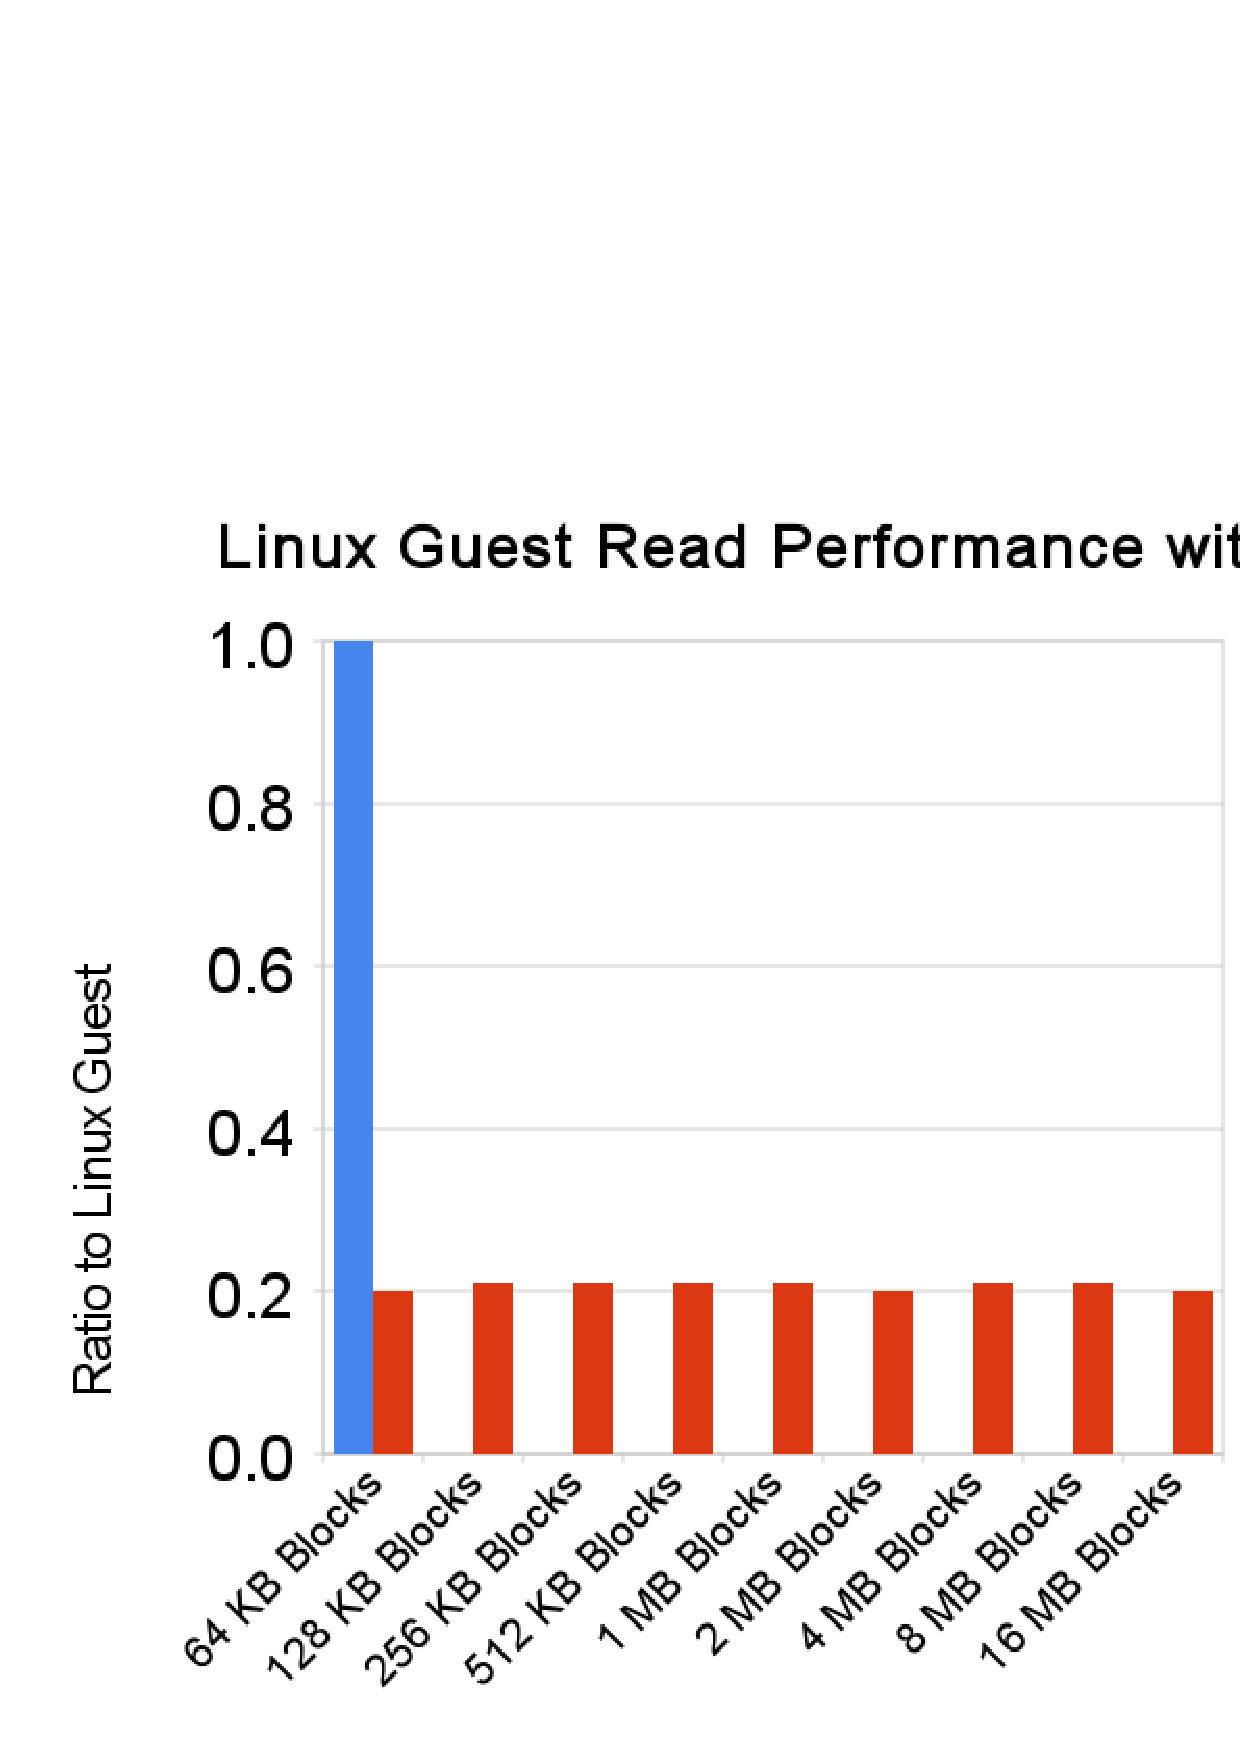
\includegraphics[scale=.7,angle=90]{figs/fs-vm-read}
\end{centering}
\end{figure}

\begin{figure}[tbp]
\begin{centering}
\rotcaption{Linux guest to FS-VM write performance}
\label{fig:fs-vm-write}
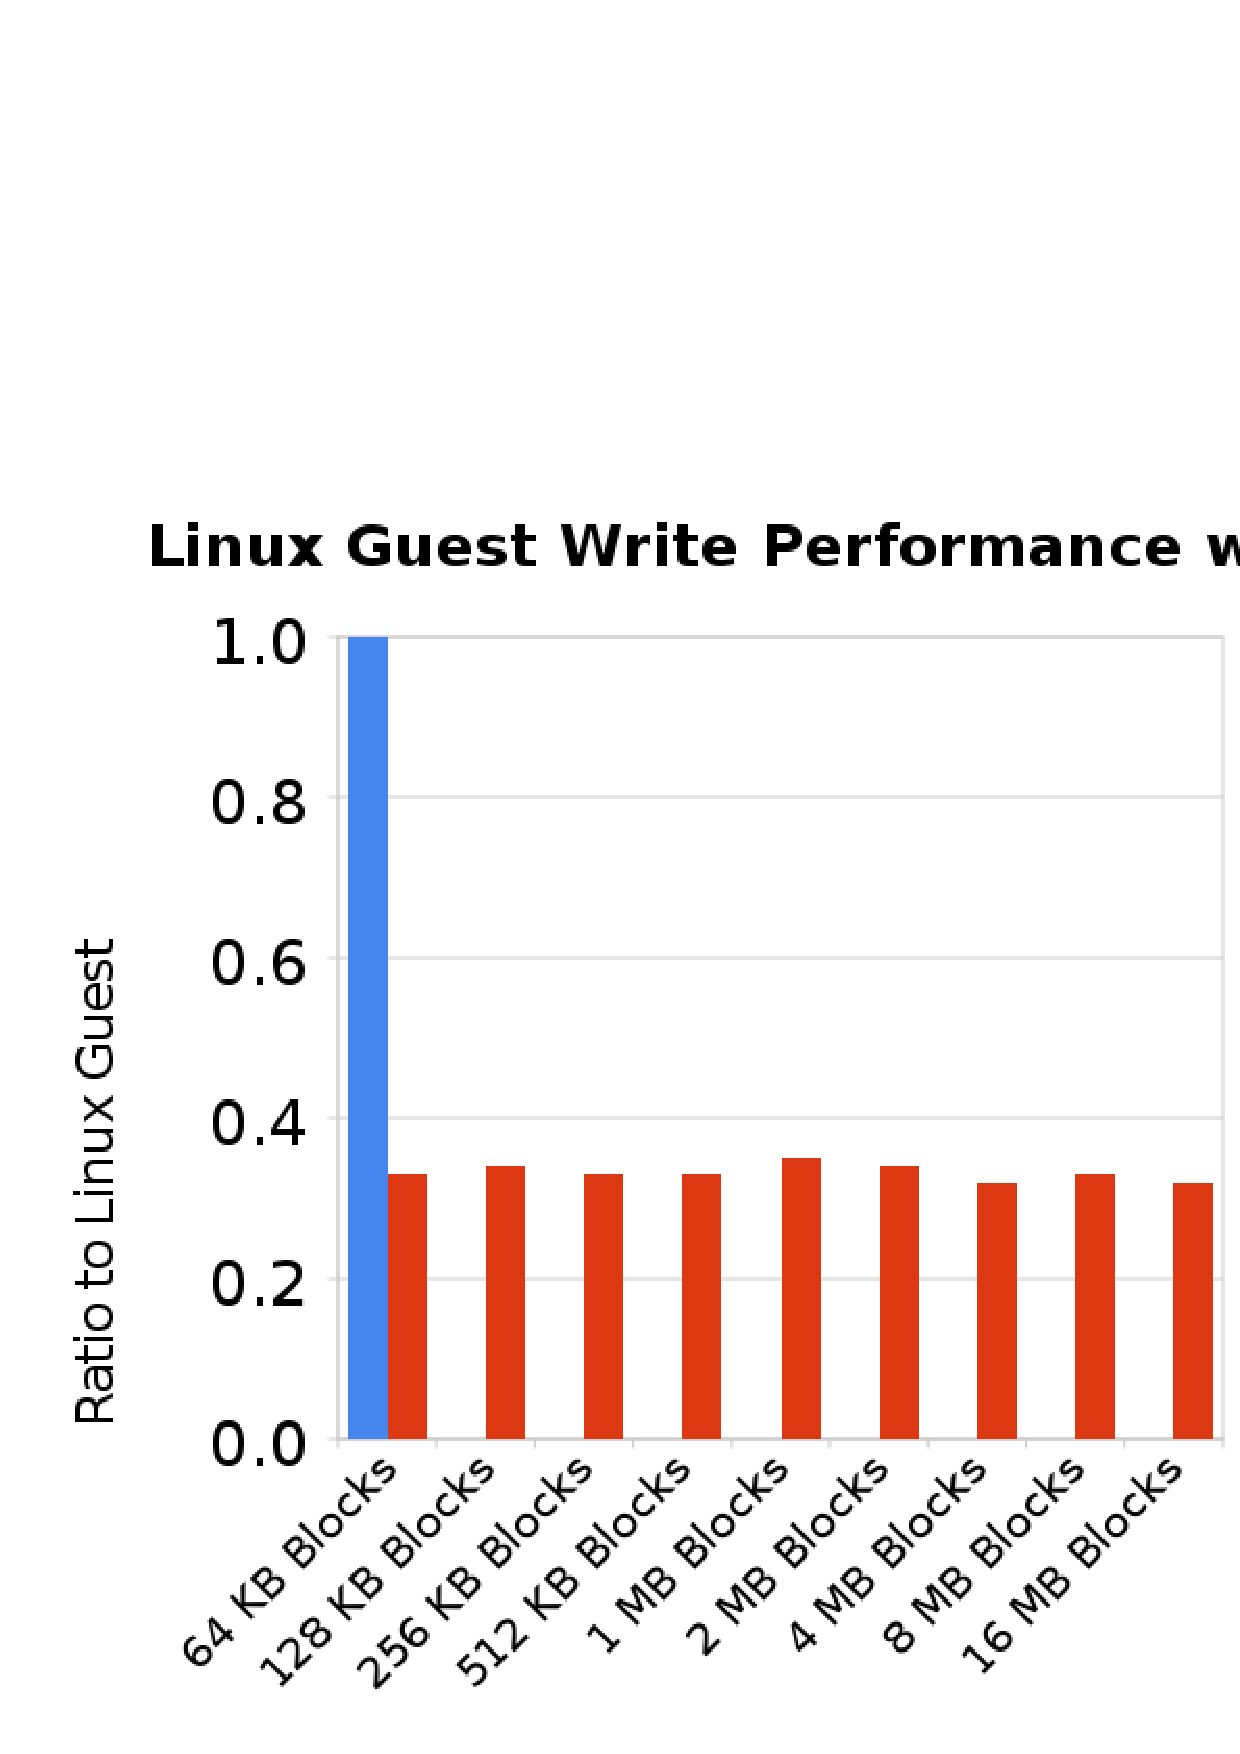
\includegraphics[scale=.7,angle=90]{figs/fs-vm-write}
\end{centering}
\end{figure}

The FS-VM as described in section \ref{sec:fs-vm-implementation} uses a qcow2 disk, but using a LVM logical volume could improve performance. More investigation is needed. We don't innovate on the FS-VM in this dissertation, but in section \ref{sec:FutureWork}, we discuss some other ways that the FS-VM could be improved.

\subsubsection{NET-VM Overhead}

Our NET-VM implementation, as described in \ref{sec:net-vm-implementation}, use OpenFlow control rules to explicitly allow flows to and from virtual appliances. To measure the overhead added by these rules we compare the network throughput of a Linux guest with and without the OpenFlow control rules protecting it. Figure \ref{fig:linux-network-ovs} shows that that average overhead added by the NET-VM component is 26\%. This is likely to be an acceptable overhead in practice, by it is also likely to improve over time with newer version of Open vSwitch, since the Open vSwitch project is still maturing. Other possible areas of improvement for the NET-VM component are discussed in the future work section of Chapter 6.

\begin{figure}[tbp]
\begin{centering}
\rotcaption{Linux guest networking performance}
\label{fig:linux-network-ovs}
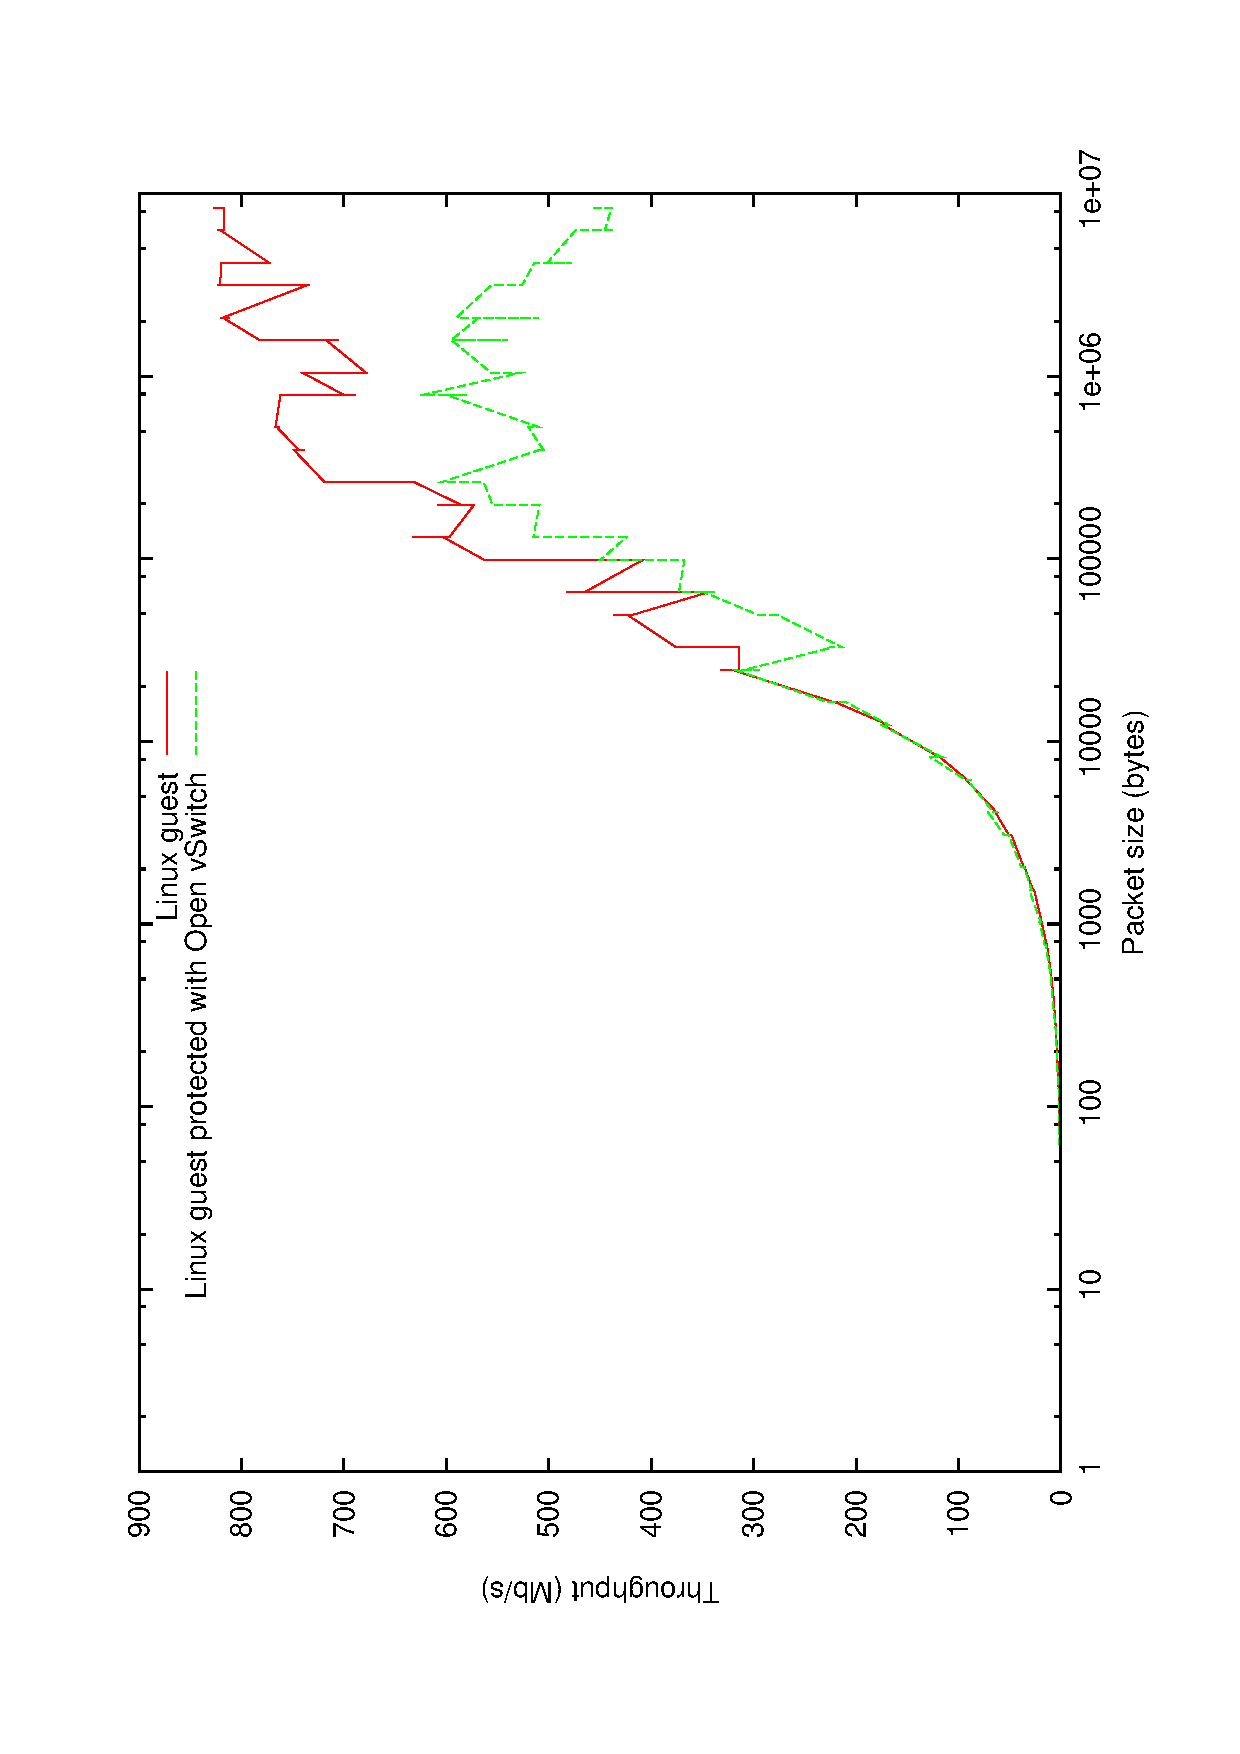
\includegraphics[scale=.7]{figs/linux-network-ovs}
\end{centering}
\end{figure}

\section{Effectiveness}
\label{sec:effectiveness}

The next evaluation criteria we consider is effectiveness. In order to measure the effectiveness of our Rapid Recovery Desktop system, we first perform an analytic evaluation of the system based on a thorough study of malware in the literature. Then, we consider various real world collection techniques and run some live malware against our system to validate that it protects the system as expected.

\subsection{Malware Classifcation Analysis}

Malware has had a lot of time to mature and evolve. Not only has the motivation of malicious hackers changed, but the actual techniques have progressed over time. However, malware still tends to fall into well-defined categories and for the most part simply follows the popular trends of the world. Malware will be deployed in ways that will target the most users. Users, by nature, flock to things that are popular and whatever is popular will be targeted.

Some things that are true of all malware is that there needs to be a way to either seek out or discover new targets, a method of distribution, an activation mechanism, and a payload. These commonalities are based on a worm taxonomy paper\cite{worm_taxonomy_2003} written in 2003. By looking at other taxonomies (such as DDoS\cite{DDoS_taxonomy_2004}, botnet\cite{botnet_taxonomy_2005} and more recent malware studies\cite{leet09_malware}, various techniques are used, but the commonalities remain. Therefore, although the exact details of the malware will evolve, the underlying principles are not likely to change. Thus, we are able to characterize and explore a classification of malware and discuss how our Rapid Recovery Desktop system would do when faced with the various scenarios.

Although there is not yet a completely agreed upon taxonomy, there are working groups~\cite{maec_website,capec_website,IEEE-SA_malwale_working_group_website} creating various standards and there is plenty of literature\cite{worm_taxonomy_2003, DDoS_taxonomy_2004, botnet_taxonomy_2005, stealth_malware_taxonomy_2006} that we draw upon for our classification. Our classification makes use of the worm taxonomy\cite{worm_taxonomy_2003} and builds upon it. Included in the literature is a stealthy malware taxonomy, some of the techniques addressed in that taxonomy actually fall out of the scope of the core of this dissertation, since that paper considers the the majority of the malware we describe in this paper as type 0 malware, which is the more ``mainstream'' malware found in practice today, and therefore is the responsibility of more traditional anti-virus techniques. The stealth malware in that paper is, in effect, able to hide itself in the operating system itself or virtualization layer. Some very challenging problems exist with that type of malware. For example, there is malware that hides in or modifies kernel data structures and malware that hides in hardware or the virtualization layer. In Chapter 3, we discussed hardening of the various components and also the recovery properties of our system, beyond that however, the stealth malware concepts fall outside the intended scope of this dissertation.

There are other ways to categorize malware (for example into viruses, worms, spyware and adware). However, in this dissertation, we will focus on the common phases in the operation of malware and not on categorizations of these types.

The commonalities as stated above are:

\begin{enumerate}
\item{Target discovery}
\item{Distribution method}
\item{Activation mechanism}
\item{Payload}
\end{enumerate}

These commonalities are not necessarily needed explicitly by each of the different types of malware, but we argue that these commonalities encompass all the malware that we consider in this dissertation. We now cover each in turn as they apply to our Rapid Recovery Desktop system. The ability to actively seek new targets or passively discover new targets is needed to continue the spread of malware.

\subsubsection{Target Discovery}
The methods to actively seek new targets are scanning and using various target list. Scanning involves probing random or sequential hosts for vulnerabilities. Target lists can come from a variety of sources, including pre-generated lists (obtained from public or private sources), metaservers (such as game servers or search engines), or internal lists (such as host files and browser history files). Our system can detect if a VM is initiating a scanning pattern and can help prevent a scanning pattern from reaching an uncompromised VM.

Scanning requires attempting to open a connection to another system. Virtual appliances, by default, are not allowed to open any connections that are not explicitly defined in their contracts, so scanning is limited only to the specific ports that the appliance has access to. In this way, the virtual appliance contracts force attackers to hide in legitimate activity. Even if malware is able to conceal its operation within legitimate traffic, we can use rate-limiting to at least slow down these type of attacks.

Some example appliances that have access to the external network include browser and email appliances. A browser appliance could be used to scan for web servers because its contract allows it to make outgoing web connections. Detecting scans for web servers is challenging, since scanning would appear just like a user connecting for legitimate web browsing. In general the user is unlikely to notice any performance loss, unless lots of connections are being made in a short period of time. In that case, an effective countermeasure is to limit the number of connections that can be made in a given period of time. This would force malware to scan more slowly or risk getting caught. In any case, even if some scanning is allowed, the fact that no incoming connections are allowed, the web server hit list is not able to be easily collected by malicious hackers. It would be possible for it to be sent out, but that would require posting the list via an outgoing web request. So, even though not every case is handled by our Rapid Recovery Desktop system, the user is likely unaffected and the malicious hackers are forced to work much harder to get around the system. 

Similarly, an email appliance could be used to scan for email servers because its contract allows it to send and receive email. Since users typically only interact with a small number of mail servers (for example, one for work email and one for personal email), a rule limiting the number of servers a user is allowed to interact with would prevent this type of scanning. Other more strict countermeasures could limit the programs that are allowed to check email. For instance, typically a single email client is used to access the user's email, especially if the user is using a specially-designed email appliance. A rule could be setup to only allow specific binaries to connect to email servers. We do not currently have an enforcement element for this type of protection, but adding enforcement elements based on introspection and HIDS techniques is discussed in future work. This technique could also help mitigate with the web server scanning example as well.

Allowing only specific binaries to connect to servers could be a good first step and could be accomplished by using standard host-based intrusion detection systems (HIDS), such as tripwire\cite{kim_tripwire_1994}. However, as pointed out in a prior virtualization intrustion dection research paper\cite{VMI_IDS_2003}, checking only the binaries is not enough, since malware could modify in-memory image of the program without modifying the actual application binary itself. Their system, called livewire, uses virtual machine introspection techniques~\cite{xenaccess_07,vmsafe_news_2008} to monitor in-memory structures to detect malicious modifications of running programs.

The passive discovery of new targets is accomplished by waiting for potential victims to contact it or by being a part of normal user activity. This is stealthy activity because it is not easily detected. An example of passive discovery is malware acting as an accepted service, such as a P2P client or web server, and responding to legitimate requests with malware. Typo-squatting and other techniques used in drive-by-downloads are another form of passive discovery. If the malware is on an appliance that is intended to run the service that the malware can run, then it would be challenging to detect since it may appear that it is functioning normally. One approach at detection could detect suspicious activity, such as when a virtual appliance tries to open new ports or performs scanning activity. Another counter measure could be to require that the appliance is using a trusted binary to provide the service.

\subsubsection{Distribution Method}

Malware needs a way to be dispersed in order for it to be more effective. If malware was never distributed, eventually it could all be cleaned up. The typical breakdown of possible ways that malware, or more specifically a worm, is circulated are by being self-carried, using a second channel, or being embedded in or transmitted in place of normal communication. We consider each method in turn and consider the reaction of the Rapid Recovery Desktop.

A worm that is self-carried transmits itself as part of the infection process. This typically means that the worm itself contains the payload. If a self-carried worm is able to find a way into the system by making use of legitimate means, then its mere existence may not be explicitly detected by our Rapid Recovery Desktop. However, as soon as it attempts to cause any harm it will likely cause contract violations for the virtual appliance into which it sneaked. We explicitly describe how this detection happens in section \ref{sec:payloads} on payloads.

A worm that requires a second channel, such as HTTP, FTP, or IRC, to complete the infection process is much less likely to work in our Rapid Recovery Desktop than on a standard system. Since virtual appliances are designed to be as special purpose as possible, a worm within a virtual appliance is less likely to have access to another channel. So, although a worm in a browser appliance that needs an extra HTTP connection to download another malware component may be able to obtain it over the web, it is not likely to be able to have access to other channels of communication.

Embedded worm propagation is the stealthiest of the propagation methods, in that by simply looking at the communications themselves (for example, monitoring email or web activity), the worm goes undetected. The malware gets in undetected, since it does not do anything. This is a sneaky way for a worm to propagate, but is only likely useful for passive worms, since if it used active methods, taking the time to be stealthy getting in would likely not be worth the extra effort. Embedded worm propagation is not necessarily any less effective on our Rapid Recovery Desktop, but it might be possible to use virtual machine introspection techniques to detect a worm that is pretending to be a trusted application or service. In any case, using the Rapid Recovery Desktop setup is comparable to using a standard system and putting defenses in place that monitor the virtual appliance from below could be an effective technique. This is a case where signature-based anti-virus or intrusion detection can still be needed in addition to being able to recover quickly from an attack.

\subsubsection{Activation Mechanism}

Malware is only effective if it is activated. Some malware can remain in the system for a long time and not be activated. It may require human intervention or may be programmed based on a specific date or be programmed to allow a certain amount of time to pass. Some malware analysis tools will only run for a specified amount of time to determine if a suspected suspicious binary is in fact malicious or not. These types of tools would miss malware that was activated based on time. The only sure way to detect these type of attacks is to make sure to cover all code paths. The process of completely reverse engineering a binary can be both difficult and time-consuming. 

The activation techniques typically break down into manual human activation, human activity-based activation, scheduled process activation, and self activation. Malware that requires manual human activation is typically a trojan that pretends to be something that the user might want, such as a media player plugin, picture, or game, but instead runs malicious code instead. This type of malware might simply be an executable or it might seem to be a legitimate file that exploits a vulnerability in a program, such as a word processor or other document viewer. 

Requiring a user to activate malware has become more popular since over time the operating systems mature and are not necessarily as easy to exploit directly. One recent popular example of this type of attack, as described in Chapter 1, is the drive-by download (automatic download and install of malware when visiting a website).  We discuss how our system could be used as a client honeypot in section \ref{sec:FutureWork}.

Malware can also be activated by other human-based activities, such as system login, system restart, or system updates. In these class of attacks, malware can add code into the registry, automatic scripts (such as start-up scripts), or replace commonly run applications, such as the system update program. In our Rapid Recovery Desktop system, we can use several techniques to reduce the number of activities that virtual appliances need to perform. For example, instead of shutting down a virtual appliance, it can be suspended to disk and started from a saved state. Further, by using a copy-on-write based disk, we can allow the appliance's disk image to be rolled back. Updates can also be performed on a copy-on-write disk, tested, and then easily reverted if necessary. This is a benefit in separating user data and system data, the user data can still remain intact.

Another activation technique is called scheduled process activation, which typically works by subverting commonly scheduled processes such as system updates and backups. A classic example of this type of attack was when the OpenSSH package was modified by an intruder who added a trojan horse\cite{openssh_trojan_2002}. The package was subsequently mirrored to official OpenSSH mirror sites before the intrusion was detected. Similarly, attacks against program install/update programs that fail to check for signed packages have been tricked into install a malicious package planted by attackers\cite{mac_vuln_2010}. Virtual Machine Introspection combined with host-based intrusion detection, as was described with the livewire system\cite{VMI_IDS_2003}, could be a good countermeasure against scheduled process activation-based attacks. We discuss how these types of systems could be integrated in section \ref{sec:FutureWork}.

Finally, self-activating malware, which can be the fastest spreading, is able to activate itself by exploiting known vulnerabilities in applications, such as system services. The classic, well-publicized example of this type of attack is Code Red, which exploited a known vulnerability in the Microsoft IIS Web Server. Our Rapid Recovery Desktop system is well-suited to defend against these types of attacks. The NET-VM and virtual switches only allow traffic that is explicitly specified in the VMCs of virtual appliances. We wouldn't expect that this type of malware would be able to spread very easily with our Rapid Recovery Desktop architecture, since we recommend running server software in a different virtual appliance from software that can access the network to download things. For example, a contract for a web server appliance would not include access to make outgoing connections (it would only need to service incoming requests).

Extending upon the worm taxonomy put for by Weaver, et al.\cite{worm_taxonomy_2003}, a more recent activation mechanism performs a more personalized attack. Malware distribution nodes (often compromised servers and systems that are part of a bot net) have been reportedly being very precise about what the malware that they give to victims. Specifically, they are able to give slightly different malware to each client. The concept of obfuscated binaries to attempt to trick signature-based scanners has been use for quite some time. The new techniques are customizing the malware to each specific hosts, often by taking a hardware profile of the victim computer and generating a unique activation code and unique binary for each system. Not only does this make it harder for malware defense to be able to detect patterns and signatures, but it allows the malware "vendors" to only allow their malware to run on specific computers. In other words, they are employing a similar model to that of Microsoft Windows Product Activation.

\begin{table}
\caption{Malware Distribution Mechanisms and Defenses}
\begin{center}
\begin{tabular}{|l|l|}
\hline
\bf Distribution & \bf \multirow{2}{*}{Defenses} \\
\bf Mechanisms & \\ \hline
Self-carried & None \\ \hline
Second channel & Block/limit unused ports, \\
(e.g. FTP, web, IM) & outgoing connections \\ \hline
Embedded in another & Block/limit outgoing \\
medium (e.g. email) & connections, SMTP \\ \hline
Manual propagation & \multirow{2}{*}{None} \\
by user (e.g. email) & \\ \hline
\end{tabular}
\end{center}
\end{table}

\subsubsection{Payloads}
\label{sec:payloads}
Malware is known to deliver up a wide variety of payloads, which are typically broken down into the following classes: None/non-functional, Internet remote control, spam-relays, proxy servers, Internet Denial of Service (DOS), data collection, access for sale, data damage, physical-world remote control, physical-world DOS, physical-world reconnaissance, physical-world damage, and malware maintenance. The access for sale and physical-world payloads are considered outside the scope of this dissertation since they deal primarily with human activity in the real world. However, restricting the access that the various virtual appliances have can limit the physical-world access that could be obtained by exploiting a virtual appliance. Further, virtual appliances, since they are running in virtual machines, do not generally have access to underlying hardware, such as web cameras, without granting them specific access, as would need to be done in the contracts.

\paragraph{Payload: None/Non-functional}
Although malware that has a missing or non-functional payload may seem harmless, there are at least two well-known examples of worms (the Morris worm\cite{Spafford_1989} and Slammer\cite{slammer_2003}) that still had a significant effect on through traffic and machine load. Another possible side effect is that vulnerable machines are being advertised more clearly simply by the presence of a particular malware. Contract rules for virtual appliances running within the Rapid Recovery Desktop system can help mitigate the system and network load. Virtualization systems typically have CPU limiting capabilities, either by limiting the number or speed of CPUs or by virtual CPU scheduling algorithms, and so virtual appliances could be limited in the amount of CPU that they use. Network rate limiting can also be done with the virtualization system, but it is often more practical to limit or shape the network traffic in the management domain or NET-VM, since standard traffic shaping techniques and virtual switch port configurations are often easier to work with and have better documentation.

\paragraph{Payload: Backdoors}
Malware that attempts to create a backdoor to be used for Internet remote control is not likely to be successful in our Rapid Recovery Desktop system, since we only allow incoming connections on ports that are explicitly requested in the virtual appliance contracts. The protection for this type of attack comes from the virtual switch configuration. Since a browser appliance would not be configured to listen on any ports, even if malware opened a backdoor in the browser appliance, the virtual switch would not allow any traffic to flow to that port.

Malware that attempts to create spam relays, or open mail servers used by remote malicious entities to send spam email, would be protected against by our Rapid Recovery Desktop system by the same method as preventing against backdoor attacks. The only small window of hope that a malicious hacker has in creating a spam relay in our Rapid Recovery Desktop system is by subverting a mail server appliance. Mitigation strategies that could be employed on mail server appliances would be to mail server configuration as read-only in the FS-VM and to place network rate-limiting contract rules on the mail server appliance itself.

Although not mentioned in the original worm taxonomy paper, another common payload used by malware is to embed a email client and attempt to send spam directly (perhaps connecting to known open relays set up by malware). This technique would not likely work in appliances other than the email client appliance, since other appliances would not be allowed to connect to remote mail servers. One mitigation strategy for the email client virtual appliance would be to limit the specific mail servers that the appliance is allowed to connect to, since users are likely to only use a very limited number of mail servers, perhaps one for personal and one for work. another mitigation strategy could be to use the virtual machine introspection techniques (also mentioned earlier in the is chapter) to make sure that the email client binary has not been compromised. 

A classic example of the use of proxy servers by spammers and other malicious hackers is the SoBig worm. The basic idea is to install a proxy server (HTTP, SOCKS, etc.) on victim computers across the Internet and then funnel spam and other malware through those proxy servers to avoid detection directly. This type of attack payload is also protected against by the Rapid Recovery Desktop system since only explicit incoming connections or specified ports are allowed.

\paragraph{Payload: Distributed Denial of Service}
Another type of payload that is very tricky to defend against is the Internet denial of service (DoS), which shortly after the worm taxonomy paper, became known as the distributed DOS (DDoS) attack. This type of payload is very commonly deployed, even today by botnets. The basic idea is that if enough zombie computers attempt to use a legitimate service at the same time, the service will not be able to handle the load, thus creating a denial of service to legitimate users. If the botnet contains enough zombie computers, then at the individual computer level the small amount of traffic (perhaps only a single request) is not considered suspicious activity. In order to mitigate this type of attack, service providers have resorted to using content distribution networks (CDNs), which distribute the load across a number of geo-located servers and is generally able allows the service to weather the storm. A more detailed look at the DDoS problem can be found in the DDoS taxonomy paper by Merkovic and Reiher\cite{DDoS_taxonomy_2004}.

Although our system can stop botnet command and control in its tracks when it tries to use communication channels that are not allowed by its contract, if it uses an allowed communication method, such as connecting to a web server, then it can be difficult to explicitly defend against. In particular, if malware residing on a browser appliance only makes a single request to a web server, it is difficult to distinguish that from any other normal user web request. However, some of the basic mitigation strategies still apply, as well as another potential technique based on user activity. If the service being attacked is different that the type of appliance that the malware has infected, then the attack will be blocked (as it was in the backdoor, spam relay, and embedded email payload cases). For example, a browser appliance would not be able to be a part in a SSH server DDoS (nor would it be able to be in a distributed SSH password guessing attack). On the other hand, if malware that is loaded on a zombie computer designed to perform a DDoS attack on a web server, then one possible mitigation technique is to use the virtual machine inspection technique of making sure the browser binary has not been compromised. Another possible mitigation technique would be to disallow new connections to by the browser appliance if no other user activity exists on the system. So, a computer that is not currently actively in use by the user (e.g. no keyboard or mouse activity and/or the computer is idle) would not be able to make any new outgoing request (existing downloads that they user may leave running would still be allowed to complete). We consider this protection based on user activity to be a good area for future work.

\paragraph{Payload: Data Collection and Data Damage}
Data collection and data damage payloads are explicitly protected against by FS-VM rules included in the virtual machine appliance contracts. First, if the virtual appliance doesn't have a need to access a particular type of data, then no access to that data is granted. Next, if a particular virtual appliance only needs to read from a particular type of data, then it is not given write or append access to the data. Further, read and write limiting rules could be specified in the virtual appliance contracts, so that explicit scanning of various data types is disallowed or limited. Attackers would still be able to access data that the appliance has access to and could slow down the rate of their attacks, but this makes the data collection process that much more challenging. In future work, we consider that the case that append-only access could be granted to further limit the ability of the attacker within a particular appliance. In the future work section of the Conclusion chapter, we consider the advantages of using "open" and "send to" dialogs to provide for better usability and security. Simultaneous to our idea, but in isolation of us, researchers have implemented a secure "send to" file transfer mechanism in the Qubes OS\cite{qubes-os_2010}, which is based on the Xen hypervisor.

\paragraph{Payload: Worm Maintenance}
A final payload that is in the original worm taxonomy is worm maintenance, which is simply a way for malware controllers to update their malware. For example, they may wish to update the list of email addresses, spam servers, or websites to attack. The mechanisms used to prevent against other remote access, such as blocking access over ports are also applicable to this case. Futher, if the attacker is trying to use a legitimate channel, virtual machine introspection techniques could be employed. In conclusion regardless of how the malware tries to subvert the system, it can only have, at most, the access that the virtual appliance in which it contains has, thus we've already added more protection than that of the typical system running a traditional operation system that is most common today. 

\begin{table}
\caption{Malware and Botnet Payloads and Defenses}
\begin{center}
\begin{tabular}{|l|l|}
\hline
\bf Payloads & \bf Defenses \\ \hline
Internet remote control & Block/limit unused, \\
(e.g. install backdoor) & listening ports \\ \hline
Spam-relays & Disallow/limit SMTP \\ \hline
Install HTML proxies & Disallow port listening \\ \hline
Denial-of-service & Block/limit out- \\
(e.g. HTTP requests) & going connections \\ \hline
& Data segmentation \\ %%
Data collection (e.g. & (grant VM access   \\
emails, credit cards) & on a need-to-know \\
& basis only) \\ \hline
\multirow{2}{*}{Data damage} & File access control \\
& and VM rollback \\ \hline
Malware maintenance & Block unused ports, \\
(e.g. update malware) & limit downloads \\ \hline
Scanning for other & Block/limit out- \\
vulnerable systems & going connections \\ \hline
\end{tabular}
\end{center}
\end{table}

\subsection{Evaluation of Recovery Properties} 

In our Rapid Recovery Desktop system, we save known-good checkpoints of each virtual appliance.  One important use of a known-good checkpoint is restoring a compromised virtual appliance from a trusted snapshot.  Any changes made within the virtual appliance since the checkpoint would be lost, but changes to personal data mounted from the FS-VM would be preserved.  In this way, personal data does not become an automatic casualty of the process of restoring a compromised system. The checkpoint image would provide an immediately functional computing platform with access to the user’s data store from the FS-VM.
 
Compromised virtual machine appliances can be automatically detected by anti-virus software or an intrusion detection system. In our prototype, when a compromised machine is detected, we stop and checkpoint the compromised virtual machine, restart a known-good checkpoint of the same virtual appliance. This process is nearly instantaneous, requiring only sufficient time to move copy on write disk image of the failed system image to a well-known location and change in the copy-on-write disk image of the trusted snapshot into place. It is worth noting that users can also trigger the restoration process manually if they suspect a compromise.
 
Once restarted, the system would still have the same vulnerability that was originally exploited.  To prevent future attacks, the trusted image should also be updated to patch the exploited vulnerability. The corrupted image can be saved or shipped to a system administrator for analysis and even the data stored inside could possibly be recovered.  Analysis of the corrupted image and/or secure logs collected by the virtual machine monitor\cite{king_2003} could provide clues to what needs to be modified.  During this analysis and recovery process, the user would still have a functional computing platform with access to the majority of their data. This is a significant improvement over the extended down time that is often required when restoring a compromised system today.
 
Our design also supports the ability to limit the number of automatic restarts. For example, after three restarts of a given image, any further compromise will result in stopping the virtual machine and checkpointing, but not in restarting the trusted snapshot. This type of response would be specified in the virtual appliance contracts and have the proper enforcement element in place to detect and take action.
 
Users can also use the restoration process to rollback a virtual appliance for any other reason (for example, they installed a piece of software and simply do not want to keep it in the system). Similarly, the restoration process can be used to recover from accidental system corruption (for example, from a routine patch or upgrade that introduced an instability into the system). Many users do not regularly apply patches and system upgrades because of the risk of instability. Stable checkpoints would encourage users to be compliant with upgrade requests by allowing them to easily experiment with the upgraded image. Reducing the risk of regular upgrades and patches is another subtle way in which virtual appliances enhance system security.

The current rollback mechanism is supported by qcow2 copy-on-write virtual disk images, but could also be supported by LVM snapshots. We discuss related enhancements to the FS-VM in section \ref{sec:FutureWork}.

